% -------------------------------------------------------------------
%  Instituto Federal do Pará
%  Campus Itaituba
%  Adaptado do pacote abntex2 http://code.google.com/p/abntex2/
%  Por Bruno Eduardo Gomes Barreto & Eliesio Alves da Silva 
% -------------------------------------------------------------------
\documentclass[
	12pt,			% tamanho da fonte
	openright,		% capítulos começam em pág ímpar (insere página vazia caso preciso)
	oneside,	
	a4paper,		% tamanho do papel.
	% -- opções da classe abntex2 --
	chapter=TITLE,	% títulos de capítulos convertidos em letras maiúsculas
    english,
    brazil
]{Sys/abntex2/abntex2} % Entre chaves vai o caminho para o arquivo .cls

%%% Pacotes utilizados %%%
% ---
% Pacotes básicos
% ---
\usepackage{bookmark}       % Usa a fonte Bookman Old Style
\usepackage[utf8]{inputenc} % permite edição direta com acentos
\usepackage[brazil]{babel}  % hifenização e títulos em português do Brasil
\usepackage[T1]{fontenc}	% Selecao de codigos de fonte.
\usepackage{color}			% Controle das cores
\usepackage{helvet}
\renewcommand{\familydefault}{\sfdefault}
\usepackage{float}
\usepackage{xurl}
\usepackage{url}
\usepackage{enumerate}
\usepackage[euler]{textgreek}
\usepackage{pdfpages}
\usepackage{csquotes}
\usepackage{lipsum}
\usepackage{textcomp}
\usepackage{parskip}
\DisemulatePackage{setspace}

%%%    IMAGENS
\usepackage{array}
\usepackage{graphicx}		% Inclusão de gráficos
\graphicspath{{imagens/}}

%%%    TABELAS E QUADRO
\usepackage{tabularx,ragged2e}	% Para inserir tabelas
\usepackage{multirow}			% Para mesclar células
\usepackage[dvipsnames,table,xcdraw]{xcolor}		% Permite adicionar cores nas linhas de tabelas
\usepackage{amsfonts}			% Permite usar notação de conjuntos
\usepackage{amsmath}			% Permite citar equações
\usepackage{amsthm}				% Permite criar teoremas e experimentos
%\usepackage[font={bf, small}, labelsep=endash, labelfont=bf]{caption}	% Faz legenda de figuras ficarem em negrito
\usepackage[font={small}, labelsep=endash]{caption}	% Faz legenda de figuras ficarem em negrito


% -------------------------------------------------
% Pacotes para QUDROS    -     funciona
% -------------------------------------------------
%\newcommand{\autodot}{}%comando criado para anular o erro
%\usepackage{tocbibind}
%\usepackage{tocbasic}
%\DeclareTOCStyleEntries{tocline}{figure,table}% now controlled by tocbasic
%\DeclareNewTOC[%
%    type=quadro,%
%    float, % define a floating environment
%    name=Quadro, %
%    listname={LISTA DE QUADROS}, %
%    setup=totoc,    % entry in ToC
%    tocentryindent:=figure,% same indentation as for figure
%    tocentrynumwidth:=figure,% same numwidth as for figure
%    floattype=4,%
%]{loq}
%\setuptoc{loq}{chapteratlist}
%%%Colocando este comando resolve o problema da lista contudo cria outro erro

\usepackage{cancel}				% Permite fazer expressão tendendo a zero
\usepackage{epstopdf}			% Converte eps para pdf

%%%    índex
\usepackage[imakeidx]{knowledge}
\indexsetup{othercode=\small}
\makeindex[program=makeindex,columns=1,intoc=true,options={-s 0_prepos/indexStyle.ist}]
\makeatletter
\def\@idxitem{\par\hangindent 0pt}
\makeatother

%%%%%%%%% NOVO
\usepackage{microtype} 	% para melhorias de justificação
\usepackage{setspace}
\urlstyle{same}
\usepackage{indentfirst} % Indenta o primeiro parágrafo de cada seção.

%%%    tabelas - configuração
\usepackage{booktabs}
\usepackage{siunitx}
\usepackage{lscape}

%%%     hifenização do português para o preambulo
\usepackage{geometry}
\usepackage{hyphenat}
\tolerance=9000

%%% lista de abreviações e siglas automática 
% -------------------------------------------------
% CONFIGURAÇÃO DE CAPÍTULOS E SEÇÕES
% -------------------------------------------------
\usepackage{titlesec}
% --------- Capítulo
\titleformat{\chapter}
    {\centering\normalfont\sffamily\bfseries\MakeUppercase}{\thechapter}{0em}{}
\titlespacing{\chapter}{0em}{0em}{3em}
% --------- Seção
\titleformat{\section}
    {\normalfont\sffamily\normalsize\bfseries}{\thesection}{0.5em}{}
\titlespacing{\section}{0em}{1.5em}{1.5em}
% --------- Subseção
\titleformat{\subsection}
    {\normalfont\sffamily\normalsize}{\thesubsection}{0.5em}{}
\titlespacing{\subsection}{0em}{1.5em}{0em}

% ------------------------------------------------
% Glossário, Index
% -------------------------------------------------
\usepackage[
    record=hybrid,
    symbols,
    abbreviations,
    acronym,
    toc,
    automake,
    xindy={language=portuguese},
    postdot,
    nonumberlist
]{glossaries-extra}
\usepackage{glossary-longbooktabs}
\usepackage{glossaries-extra-stylemods}
\usepackage{glossary-inline}
\setglossarystyle{list}
\glssetcategoryattribute{general}{indexname}{textbf}
\glssetcategoryattribute{general}{dualindex}{true}
\glssetcategoryattribute{abbreviation}{indexname}{textbf}
\glssetcategoryattribute{abbreviation}{dualindex}{true}
\glssetcategoryattribute{general}{glossname}{firstuc}
\GlsXtrEnableIndexFormatOverride
\renewcommand*{\glsxtrautoindexentry}[1]{\string\glsentryfirst{#1}}
\renewcommand*{\glsxtrautoindexassignsort}[2]{%
  \ifglshaslong{#2}%
  {\glsletentryfield{#1}{#2}{long}}%
  {\glsletentryfield{#1}{#2}{sort}}%
}
\makeglossaries
\renewcommand*{\glsnamefont}[1]{%
    \textmd{#1}:%
}
% PADRÃO DE ENTRADA NO GLOSSÁRIO
%\newglossaryentry{aPalavra}{
%        name= {APALVRA},       %%% EM CAIXA ALTA, É O QUE IRÁ APARECER NO GLOSSÁRIO, PARA SEGUIR A NORMA DO IFPA
%        text = {aPalavra},    %%% como irá aparecer no TEXTO
%        sort = {Formula},     %% REESCREVA A PALAVRA SEM USAR NENHUMA ACENTUAÇÃO PARA QUE POSSA SER USADA PARA ORGANZIAR O GLOSSÁRIO
%        description={É uma linguagem de marcação especialmente feita para documentos científicos}              %DESCRIÇÃO
%}
%
% ADICIONE AS ENTRADAS USANDO A ORDEM ALFABÉTICA
%

\newglossaryentry{fórmula}{
        name = {FÓRMULA},
        text = {fórmula},
        sort = {Formula},     %% PALAVRA ACENTUADAS DEVERÃO CONTER O CAMPO 'SORT' PARA AJUDAR NA ORDENAÇÃO 
        description={Uma expressão matemática}
}

\newglossaryentry{latex}{
        name= {LATEX},
        text = {latex},
        sort = {latex},
        description={É uma linguagem de marcação especialmente feita para documentos científicos}
}

\newglossaryentry{matemática}{
        name = {MATEMÁTICA},
        text = {matemática},
        sort = {matematica},
        description={Matemática é o que a matemática faz}
}

\longnewglossaryentry{sample}{
    name = {SAMPLE},
    text = {sample},            % -    versão em texto
    plural = {samples},         %  -    versão em plural no texto
    sort = {sample},
}{%
     {an example}       %DESCRIÇÃO
}

%\newterm[〈key=value list〉]{〈entry-label〉}
%This is just a shortcut that uses \newglossaryentry with the name set to 〈entry-label〉 and
%the description is suppressed.


%\newglossaryentry{not:set}
%{% This entry goes in the `notation' glossary:
%type={notation},
%name={$\mathcal{S}$},
%text={\mathcal{S}},
%description={A set},
%sort={S}
%}

% -------------------------------------------------
% abreviações e siglas
% -------------------------------------------------
\usepackage{acro}
%%%  LISTA DE ABREVIAÇÕES e SIMBOLOS
% no decorrer da sua escrita, você usará abreviações e símbolos
% estes simbolos e abreviações devem constar na lista de abreviações
% e simbolos. Para gerar AUTOMATICAMENTE estas listas sem o menor esforço 
% você deve declarar NESTE documento todas as ABREVIAÇÕES e todos os SÍMBOLOS
% que você usará no decorrer do texto. 
% 
% SOMENTE DEPOIS DE DECLARAR AQUI
%
% você será capaz de pôr o simbolo usando a biblioteca ACRONYM
%
% usando os comandos        \ac      e     \acl
%	
%	 Para utilizar abreviaturas e simbolos, basta utilizar o comando barra \ combinado com ac ou acl.
%	 
%	 Abreviaturas e a versão por extenso.
%	 
%	 AC \ac{abntex}.     MOSTRARÁ A ABREVIAÇÃO
%%	 
%	 ACL \acl{abntex}.   MOSTRARÁ AS PALAVRAS DA ABREVIAÇÃO POR EXTENSO
%	 
%%	 Simbolos e a versão por extenso.
%	 
%	 AC  \ac{lambda}.   MOSTRARÁ O SIMBOLO
%	 
%	 ACL \acl{lambda}.  MOSTRARÁ A PALAVRA DO SIMBOLO POR EXTENSO
% 
% class `abbrev': abbreviations:
%NOTE QUE SOMENTE OS QUE SÃO CHAMADOS NO DECORRER DO TEXTO IRÃO APARECER NA LISTA DE ABREVIATURAS E SIMBOLOS
%PADRÃO PARA ABREVIATURA

%\DeclareAcronym{}{
%	short = \normalfont{},
%	long  = \textit{},
%	class = abbrev
%}

\DeclareAcronym{sbc}{
	short = \normalfont{SBC},
	short-plural = s,
	long  = Sociedade Brasileira de Computação,
	tag = abbrev
}

\DeclareAcronym{nc}{
	short = \normalfont{NC},
	long  = \textit{Networking Coding},
	tag = abbrev
}

\DeclareAcronym{abnt}{
	short = \normalfont{ABNT},
	short-plural = s,
	long  = Associação Brasileira de Normas Técnicas,
	tag = abbrev
}

\DeclareAcronym{abntex}{
	short = \normalfont{abnTeX},
	short-plural = s,
	long  = ABsurdas Normas para TeX,
	tag = abbrev
}


%%%  LISTA DE SIMBOLOS
%PADRÃO PARA SIMBOLO
%\DeclareAcronym{}{
%	short = \normalfont{},
%	long  = \textit{},
%   sort = ,
%	tag = nomen
%}

\DeclareAcronym{megaByte}{
	short = \normalfont{MB},
	long  = é uma unidade de medida de informação que equivale a 1000000 bytes,
	sort  = MB,
	tag = nomen,
}

\DeclareAcronym{lambda}{
	short = \normalfont{\textlambda} ,
	long  = comprimento de onda,
	sort  = \textlambda,
	tag = nomen,
}

% -------------------------------------------------
%%%%%% estilo do capítulo
%%%%%% escolha 1 e tire o comentário
%% acesse a página e escolha
%%http://ctan.math.washington.edu/tex-archive/info/latex-samples/MemoirChapStyles/MemoirChapStyles.pdf
% -------------------------------------------------
\setlength\midchapskip{12pt}
%%%%%%%%   CAPA
\instituicao{INSTITUTO FEDERAL DE EDUCAÇÃO, CIÊNCIA E TECNOLOGIA DO PARÁ}

%%%%%% caso esteja envolvido em algum plano ou programa de pós-graduação de curso específico, 
%% preencha o comando abaixo
\plano{}

\campus{CAMPUS ITAITUBA}

\curso{TECNÓLOGO EM ANÁLISE E DESENVOLVIMENTO DE SISTEMAS}

%(use \\ para separar os autores)
\autor{
    NOME DOS ALUNOS EM CAIXA ALTA
    \\
    OUTRO FULANO DE TAL DA CASA QUEBRADA
    \\
    OUTRO FULANO DE TAL DA CASA ARRUMADA
    \\
    NOME DO OUTRA AUTOR EM CAIXA ALTA AO QUADRADO
    \\
    OUTRO FULANO DE TAL DA CASA BONITA
}

\titulo{NOME DA TESE, DISSERTAÇÃO OU TCC EM CAIXA ALTA}

\tipotrabalho{Monografia}

\local{ITAITUBA}

\data{2023}

%%%%%%%%   CONTRACAPA

\orientador[Orientador(a)]{Prof.\textdegree \space Dr. Fulano de Tal}%Nome e titulação do(a) professor(a) orientador(a)}

%%%% COLOQUE O MESMO TEXTO EM AMBOS

% O preambulo deve conter o tipo do trabalho, o objetivo, 
% o nome da instituição e a área de concentração 

\hyphenation{
    Trabalho de conclusão de curso apresentado ao Instituto Federal de Ciência e Tecnologia do Pará - IFPA Campus Itaituba como requisito para obtenção de grau em Tecnólogo em Análise e Desenvolvimento de Sistemas.
}
\preambulo{
    Trabalho de conclusão de curso apresentado ao Instituto Federal de Ciência e Tecnologia do Pará - IFPA Campus Itaituba como requisito para obtenção de grau em Tecnólogo em Análise e Desenvolvimento de Sistemas.
}

% -------------------------------------------------
% Informações do PDF
% -------------------------------------------------
\makeatletter
\hypersetup{
    colorlinks=true,
    linkcolor=blue,
    citecolor=blue,
    filecolor=magenta,      
    urlcolor=blue,
    bookmarksopen=true,
    %pagebackref=true,
	pdftitle={\imprimirtitulo}, 
	pdfauthor={\imprimirautor},
    pdfsubject={\imprimirpreambulo},
    pdfcreator={LaTeX with abnTeX2},
	pdfkeywords={\imprimirpalavraschave}{trabalho acadêmico},
	bookmarksdepth=4,
    breaklinks=true,
}
\makeatother

% -------------------------------------------------
% Espaçamentos entre linhas e parágrafos 
% -------------------------------------------------
% O tamanho do parágrafo é dado por:
\setlength{\parskip}{0.0cm}
\setlength{\parindent}{1.0cm}
\renewcommand{\baselinestretch}{1.5}
\renewcommand*{\afterchapskip}{1.5ex}

% -------------------------------------------------
% Referências Bibliográficas se dá pela pasta abnt
% e a seguinte biblioteca
% -------------------------------------------------
\usepackage{hyperref}
\usepackage[brazilian,hyperpageref]{backref}	 % Paginas com as citações na bibl
\usepackage{breakurl}
\usepackage[
        versalete,
        abnt-emphasize = bf, % destaca o titulo da revista ou livro em negrito;
        abnt-etal-list = 3, % trabalhos com mais de 3 autores recebem et al.,;
        abnt-etal-text = it, % escreve o et al., em italico;
        abnt-and-type = &, % usa o carater '&' no lugar de 'e' para mais de um autor;
        abnt-last-names = abnt, % trata sobrenomes 'estritamente' conforme a ABNT; e
        abnt-repeated-author-omit = no, % autores com + de uma entrada recebem '____.',
        alf
%        abnt-url-package = url
        ]{abntex2cite}
\usepackage{Sys/0_prepos/url6023}

% -------------------------------------------------
% Biblioteca para adicionar CÓDIGO
% -------------------------------------------------
\usepackage{listings}
\usepackage{xcolor}
\definecolor{codegreen}{rgb}{0,0.6,0}
\definecolor{codegray}{rgb}{0.5,0.5,0.5}
\definecolor{codepurple}{rgb}{0.58,0,0.82}
\definecolor{backcolour}{rgb}{0.95,0.95,0.92}
\lstdefinestyle{mystyle}{
    backgroundcolor=\color{backcolour},   
    commentstyle=\color{codegreen},
    keywordstyle=\color{magenta},
    numberstyle=\tiny\color{codegray},
    stringstyle=\color{codepurple},
    basicstyle=\ttfamily\footnotesize,
    breakatwhitespace=true,
    escapeinside={\%*}{*)},  % if you want to add LaTeX within your code
    keepspaces=true,  % keeps spaces in text
    mathescape=true,
    breaklines=true,
    caption={Código},
    captionpos=t,
    numbers=left,                    
    numbersep=2pt,                  
    stepnumber=1,
    numberstyle=\tiny,
    numbersep=10pt,
    showstringspaces=false,
    showtabs=false,                  
    tabsize=2,
    extendedchars=true,
    inputencoding=utf8,
    literate={á}{{\'a}}1  {é}{{\'e}}1  {í}{{\'i}}1 {ó}{{\'o}}1  {ú}{{\'u}}1 {Á}{{\'A}}1  {É}{{\'E}}1  {Í}{{\'I}}1 {Ó}{{\'O}}1  {Ú}{{\'U}}1 {à}{{\`a}}1  {è}{{\`e}}1  {ì}{{\`i}}1 {ò}{{\`o}}1  {ù}{{\`u}}1 {À}{{\`A}}1  {È}{{\'E}}1  {Ì}{{\`I}}1 {Ò}{{\`O}}1  {Ù}{{\`U}}1 {ä}{{\"a}}1  {ë}{{\"e}}1  {ï}{{\"i}}1 {ö}{{\"o}}1  {ü}{{\"u}}1 {Ä}{{\"A}}1  {Ë}{{\"E}}1  {Ï}{{\"I}}1 {Ö}{{\"O}}1  {Ü}{{\"U}}1 {â}{{\^a}}1  {ê}{{\^e}}1  {î}{{\^i}}1 {ô}{{\^o}}1  {û}{{\^u}}1 {Â}{{\^A}}1  {Ê}{{\^E}}1  {Î}{{\^I}}1 {Ô}{{\^O}}1  {Û}{{\^U}}1 {œ}{{\oe}}1  {Œ}{{\OE}}1  {æ}{{\ae}}1 {Æ}{{\AE}}1  {ß}{{\ss}}1 {ç}{{\c c}}1 {Ç}{{\c C}}1 {ø}{{\o}}1  {Ø}{{\O}}1   {å}{{\r a}}1 {Å}{{\r A}}1 {ã}{{\~a}}1  {õ}{{\~o}}1 {Ã}{{\~A}}1  {Õ}{{\~O}}1 {ñ}{{\~n}}1  {Ñ}{{\~N}}1  {¿}{{?`}}1  {¡}{{!`}}1 {°}{{\textdegree}}1 {º}{{\textordmasculine}}1 {ª}{{\textordfeminine}}1,
    frame=single,
    framerule=0pt,
    framesep=-2pt,
    rulesep=0pt,
    rulecolor=\color{black},
    showspaces=false,
    %nolol=false,
    numberbychapter=false,
}
\lstset{style=mystyle}
\usepackage[hypcap]{caption}
\DeclareCaptionLabelFormat{bf-parens}{(\textbf{#2})}
\captionsetup[lstlisting]{singlelinecheck=false, labelsep=endash}
\renewcommand\lstlistingname{Código}
\renewcommand\lstlistlistingname{Lista de Códigos}


% -------------------------------------------------
% Padrão para CAPA e CONTRACAPA
% -------------------------------------------------
\geometry{a4paper, left=3cm, right=2cm, top=3cm, bottom=2cm, headheight=0.5cm, textheight=44\baselineskip, headsep=0.01cm}

% -------------------------------------------------
% Pacotes para sumário
% -------------------------------------------------
\usepackage{tocloft}

%8888888888888888888888888888888888888888888888888888
%            ACRESCENTADOS POR ELIESIO
%8888888888888888888888888888888888888888888888888888
\usepackage{tcolorbox}
\usepackage{pifont}
\usepackage{tikz}
\newcommand{\ajuda}{
\begin{tcolorbox}[colback=blue!5!white,colframe=red!25!blue,title= Comando de Ajuda]
Digite os comandos em \textcolor{red}{Vermelho} para obter a ajuda desejada.\\[5pt]
\textcolor{red}{$\backslash$estruturaDoc} Para ajudá-lo com a estrutura do seu documento; \\[5pt]
\textcolor{red}{$\backslash$upArquivos} Para ajudá-lo com o Upload de arquivos para o overleaf; \\[5pt]
\textcolor{red}{$\backslash$fazerLista} Para ajudá-lo a  fazer uma lista numerada ou não; \\\textcolor{red}{$\backslash$adicionaFormula} Para ajudá-lo a adicionar uma equação matemática numerada ou não; \\[5pt]
\textcolor{red}{$\backslash$adicionaCodigo} Para ajudá-lo na adição de um Código;\\
\textcolor{red}{$\backslash$adicionaQuadro} Para ajudá-lo na adição de um Quadro;\\
\textcolor{red}{$\backslash$adicionaTabela} Para ajudá-lo na adição de uma Tabela;\\
\textcolor{red}{$\backslash$adicionaFig} Para ajudá-lo na adição de uma figura; \\[5pt]
\textcolor{red}{$\backslash$letrasGregas} Para ajudá-lo na adição de caracteres gregos;\\
\textcolor{red}{$\backslash$caracterEspecial} Para ajudá-lo na adição de caracteres especiais;\\
\textcolor{red}{$\backslash$adicionaSigla} Para ajudá-lo na adição de uma Sigla;\\
\textcolor{red}{$\backslash$adicionaSimbolo} Para ajudá-lo na adição de um Simbolo;\\
\textcolor{red}{$\backslash$adicionaPalavraGlossario} Para ajudá-lo na adição de uma Palavra ao Glossário;\\[10pt]
Quando não precisar mais de ajuda, comente a linha \textcolor{blue}{$\backslash$ajuda} \texttt{ - para comentar digite o caracter \% antes do comando. Ex. \textcolor{black!40!white}{\%$\backslash$ajuda}}
\end{tcolorbox}
}

\newcommand{\adicionaFormula}{
\begin{tcolorbox}[colback=blue!5!white,colframe=black!25!pink,title= Comandos básicos utilizados para acrescentar equações numeradas ou não]
\ding{42} Formas de adicionar uma equação não numerada:\\[5pt]
\ding{172} No meio de texto; 
$$\text{texto1} \$\texttt{equação}\$\text{ texto2}$$
Ex. O teorema \$c\^{}2 = a\^{}2 + b\^{}2\$ a seguir $\Rightarrow$  O teorema $c^2 = a^2 + b^2$ a seguir\\[5pt]
\ding{173} Centralizado em linha separada
$$\$\$\text{ equação }\$\$$$
Ex. \$\$\textcolor{blue}{$\backslash$displaystyle $\backslash$sum}\_\{i=1\}\^{}n f\textcolor{blue}{$\backslash$left}(x\_i\textcolor{blue}{$\backslash$right})\$\$ quando compilado
$$\displaystyle \sum_{i=1}^nf\left(x_i\right)$$
\ding{42} Formas de adicionar uma equação numerada:\\[5pt]
\textcolor{blue}{$\backslash$begin}\{equation\} \texttt{ - inicia o ambiente equação}\\
\textcolor{blue}{$\backslash$displaystyle $\backslash$int}\_a\^{}b f(x)dx = F(b) - F(a) \texttt{ - equação}\\
\textcolor{blue}{$\backslash$label}\{eq:cap1eq1\} \texttt{ - rótulo da equação no documento}\\
\textcolor{blue}{$\backslash$end}\{equation\} \texttt{ - finaliza o ambiente equação}\\[10pt]
Quando compilada a equação \ref{eq:cap1eq1} ficaria
\begin{equation}
    \displaystyle \int_a^bf(x)dx=F(b)-F(a)
    \label{eq:cap1eq1}
\end{equation}
\ding{96} necessário no caso de referenciar em outra parte do documento\\
Para não exibir numeração \textcolor{blue}{$\backslash$begin}\{equation*\} $\ldots$ \textcolor{blue}{$\backslash$end}\{equation*\}\\[5pt]
Para a equação à esquerda modifique as configurações no preambulo (antes dos pacotes) \textcolor{blue}{$\backslash$documentclass}[fleqn]\{classe do documento\}
\end{tcolorbox}
}

\newcommand{\estruturaDoc}{
\begin{tcolorbox}[colback=blue!5!white,colframe=black!25!yellow,title= Comandos básico utilizados na estrutura desse documento]
Principais comando utilizados na estrutura hierárquica desse documento:\\[5pt]
\textcolor{blue}{$\backslash$chapter}\{título do capítulo\}\texttt{ - para abreviar no sumário utilize ``$\backslash$chapter[título abreviado]\{título do capítulo\}'' sem aspas}\\
\textcolor{blue}{$\backslash$section}\{título da seção\}\texttt{ - texto do segundo nível}\\
\textcolor{blue}{$\backslash$subsection}\{título da subseção\}\texttt{ - texto do terceiro nível}\\
\textcolor{blue}{$\backslash$subsubsection}\{título do 4\textdegree~ nível\}\\[10pt]
Capítulos, seções, subseções e subsubseções podem ser rotulados, logo abaixo da entrada do capítulo, para eventuais chamadas em outras partes do documento.\\[10pt]
\textcolor{blue}{$\backslash$label}\{sec:introdução\}\texttt{ - exemplo de entrada do rótulo de chamada da introdução}\\[10pt]
\textcolor{blue}{$\backslash$ref}\{sec:introdução\} \texttt{ - quando digitado no documento, faz a referência ao capítulo introdução} 
\end{tcolorbox}
}
\newcommand{\caracterEspecial}{
\begin{tcolorbox}[colback=blue!5!white,colframe=red!25!yellow,title= Comandos para caracteres especiais]
Para adicionar um caracter especial digite um dos comando em \textcolor{blue}{azul} abaixo:\\[5pt]
\begin{tabular}{lclp{3cm}rcl}
\textcolor{blue}{$\backslash$\$}&\texttt{-  para -}&\$&&\textcolor{blue}{$\backslash$\&}&\texttt{-  para -}&\&\\
\textcolor{blue}{$\backslash$\%}&\texttt{-  para -}&\%&&\textcolor{blue}{$\backslash$\#}&\texttt{-  para -}&\#\\
\textcolor{blue}{$\backslash$\_}&\texttt{-  para -}&\_&&\textcolor{blue}{$\backslash$\{}&\texttt{-  para -}&\{\\
\textcolor{blue}{$\backslash$\}}&\texttt{-  para -}&\}&&\textcolor{blue}{$\backslash$\~{}\{\}}&\texttt{-  para -}&\~{}\\
\textcolor{blue}{$\backslash$\^{}\{\}}&\texttt{-  para -}&\^{}&&\textcolor{blue}{\$$\backslash$backslash\$}&\texttt{-  para -}&$\backslash$\\
\end{tabular}
\end{tcolorbox}
}

\newcommand{\letrasGregas}{
\begin{tcolorbox}[colback=blue!5!white,colframe=red!75!yellow,title= Comandos para caracteres gregos]
Para adicionar uma letra grega digite um dos comando em \textcolor{blue}{azul} abaixo:\\[5pt]
\begin{tabular}{lcl}
\textcolor{blue}{$\backslash$alpha} \texttt{-  para a letra \alpha}&&\textcolor{blue}{$\backslash$beta} \texttt{-  para a letra \beta}\\
\textcolor{blue}{$\backslash$gamma} \texttt{-  para a letra \gamma}&&\textcolor{blue}{$\backslash$delta} \texttt{-  para a letra \delta}\\
\textcolor{blue}{$\backslash$epsilon} \texttt{-  para a letra \epsilon}&&\textcolor{blue}{$\backslash$varepsilon} \texttt{-  para a caracter \varepsilon}\\
\textcolor{blue}{$\backslash$zeta} \texttt{-  para a letra \zeta}&&\textcolor{blue}{$\backslash$eta} \texttt{-  para a letra \eta}\\
\textcolor{blue}{$\backslash$theta} \texttt{-  para a letra \theta}&&\textcolor{blue}{$\backslash$vartheta} \texttt{-  para o caracter \vartheta}\\
\textcolor{blue}{$\backslash$iota} \texttt{-  para a letra \iota}&&\textcolor{blue}{$\backslash$kappa} \texttt{-  para a letra \kappa}\\
\textcolor{blue}{$\backslash$lambda} \texttt{-  para a letra \lambda}&&\textcolor{blue}{$\backslash$mu} \texttt{-  para a letra \mu}\\
\textcolor{blue}{$\backslash$nu} \texttt{-  para a letra \nu}&&\textcolor{blue}{$\backslash$xi} \texttt{-  para a letra \xi}\\
\textcolor{blue}{o} \texttt{-  para a letra ômicron}&&\textcolor{blue}{$\backslash$pi} \texttt{-  para a letra \pi}\\
\textcolor{blue}{$\backslash$varpi} \texttt{-  para o caracter \varpi}&&\textcolor{blue}{$\backslash$rho} \texttt{-  para a letra \rho}\\
\textcolor{blue}{$\backslash$varrho} \texttt{-  para o caracter \varrho}&&\textcolor{blue}{$\backslash$sigma} \texttt{-  para a letra \sigma}\\
\textcolor{blue}{$\backslash$varsigma} \texttt{-  para o caracter \varsigma}&&\textcolor{blue}{$\backslash$tau} \texttt{-  para a letra \tau}\\
\textcolor{blue}{$\backslash$upsilon} \texttt{-  para a letra \upsilon}&&\textcolor{blue}{$\backslash$phi} \texttt{-  para a letra \phi}\\
\textcolor{blue}{$\backslash$varphi} \texttt{-  para o caracter \varphi}&&\textcolor{blue}{$\backslash$chi} \texttt{-  para a letra \chi}\\
\textcolor{blue}{$\backslash$psi} \texttt{-  para a letra \psi}&&\textcolor{blue}{$\backslash$omega} \texttt{-  para a letra \omega}
\end{tabular}\\[5pt]
Caracteres Maiúsculos\\
\begin{tabular}{lcl}
\textcolor{blue}{$\backslash$Gamma} \texttt{-  para a letra \Gamma}&&\textcolor{blue}{$\backslash$Delta} \texttt{-  para a letra \Delta}\\
\textcolor{blue}{$\backslash$Theta} \texttt{-  para a letra \Theta}&&\textcolor{blue}{$\backslash$Lambda} \texttt{-  para a letra \Lambda}\\
\textcolor{blue}{$\backslash$Xi} \texttt{-  para a letra \Xi}&&\textcolor{blue}{$\backslash$Pi} \texttt{-  para a letra \Pi}\\
\textcolor{blue}{$\backslash$Sigma} \texttt{-  para a letra \Sigma}&&\textcolor{blue}{$\backslash$Upsilon} \texttt{-  para a letra \Upsilon}\\
\textcolor{blue}{$\backslash$Phi} \texttt{-  para a letra \Phi}&&\textcolor{blue}{$\backslash$Psi} \texttt{-  para a letra \Psi}\\
\textcolor{blue}{$\backslash$Omega} \texttt{-  para a letra \Omega}&&\\
\end{tabular}
\end{tcolorbox}
}



\newcommand{\adicionaFig}{
\begin{tcolorbox}[colback=blue!5!white,colframe=green!75!blue,title= Comando Acrescenta figura, fontlower=\footnotesize]
Para adicionar uma figura no documento siga os passos abaixo:\\[5pt]
\textcolor{blue}{$\backslash$begin}\{figure\}[h!]\\
\texttt{Inicia o ambiente, o ``h!'' significa aqui, ``H'' - Ambos fixam a imagem naquela exata posição do texto}\\
\textcolor{blue}{$\backslash$setstretch\{1.5\}$\backslash$centering$\backslash$footnotesize} \\
\texttt{Configura Rodapé: espaçamento - centralização - tamanho da fonte}\\
\textcolor{blue}{$\backslash$caption}\{texto\}\texttt{ - ``texto'' é a descrição da figura no documento} \\
\textcolor{blue}{$\backslash$begin}\{center\} \texttt{centraliza a imagem}\\
\textcolor{blue}{$\backslash$includegraphics}[tamanho]\{nomeArquivo\}\\
\texttt{ - ``tamanho'' pode ser escalonado(ex. scale=0.5) ou largura(width) e altura(height), ex. width=3cm, height=0.5$\backslash$linewidth.\\
``nome.ext'' todas as imagens devem ser adicionadas na pasta ``imagens''. A ``.ext'' refere-se a extensão da imagem ex. .jpg,.png,etc}\\
\textcolor{blue}{$\backslash$end}\{center\} \texttt{Fim da centralização da Imagem}\\
\textcolor{blue}{$\backslash$label}\{fig:nomedafigura\}\texttt{ - indica como a figura será referenciada no documento}\\
\textcolor{blue}{$\backslash$par} Fonte:  local de origem \texttt{ - indica o local de origem da figura ou quem a produziu}\\
\textcolor{blue}{$\backslash$end}\{figure\}\texttt{ - finaliza o ambiente figure}
\tcblower
\textcolor{blue}{EXEMPLO}\\
$\backslash$begin\{figure\}[H]\\
\tab $\backslash$setstretch\{1.5\}$\backslash$centering$\backslash$footnotesize\\
\tab $\backslash$caption\{Album A Presenca da Gloria da banda Santa Geracao\}\\
\tab $\backslash$begin\{center\}\\
\tab \tab $\backslash$includegraphics[width=0.5$\backslash$textwidth]\{presencaDaGloria.png\}\\
\tab $\backslash$end\{center\}\\
\tab $\backslash$label\{fig:capaPresencaDaGloria\}\\
\tab $\backslash$par Fonte: Google Imagens\\
$\backslash$end\{figure\}\\
\end{tcolorbox}
}

\newcommand{\adicionaQuadro}{
\begin{tcolorbox}[colback=blue!5!white,colframe=green!75!blue,title= Comando Acrescenta Quadro, fontlower=\footnotesize]
Acesse o site: https://www.tablesgenerator.com para produzir um quadro/tabela\\
\textcolor{blue}{$\backslash$begin}\{Quadro\}[H]\texttt{ - inicia o ambiente quadros ``H'' aqui!}\\
\textcolor{blue}{$\backslash$setstretch\{1.5\}$\backslash$centering$\backslash$footnotesize} \\
\texttt{Conf. Rodapé: espaçamento|centralização|tamanho da fonte}\\
\textcolor{blue}{$\backslash$caption}\{texto\}\texttt{ - ``texto'' é a descrição do quadro}\\
\textcolor{blue}{$\backslash$begin}\{center\}\texttt{ - inicia o ambiente centralizar}\\
\textcolor{blue}{$\backslash$begin}\{tabular\}\{|c|c|\}\textcolor{blue}{$\backslash$hline}\texttt{- inicia o ambiente tabular que cria a estrutura do quadro, ``|c|c|'' são duas colunas centralizadas, ``$\backslash$hline'' insere uma linha horizontal}\\
Título Coluna1 \& Título Coluna2 \textcolor{blue}{$\backslash \backslash \backslash$hline}\texttt{ - Texto das colunas ``\&'' separa as colunas}\\
valor1 \& valor2 \textcolor{blue}{$\backslash\backslash \backslash$hline}\texttt{ - valores das colunas para uma linha. Para acrescentar mais linhas insira os valores, separados por \& e finalize com $\backslash\backslash \backslash$hline}\\
\textcolor{blue}{$\backslash$end}\{tabular\}\texttt{ - finaliza o ambiente tabular}\\
\textcolor{blue}{$\backslash$end}\{center\}\texttt{ - finaliza o ambiente centralizar}\\
\textcolor{blue}{$\backslash$label}\{qua:nome\}\texttt{ - insere um rótulo para a chamar o quadro}\\
 \textcolor{blue}{$\backslash$par} Fonte: Elaborado por \texttt{ - indica a fonte do quadro}\\
\textcolor{blue}{$\backslash$end}\{Quadro\}\texttt{ - finaliza o ambiente quadro}
\tcblower
\textcolor{blue}{EXEMPLO}\\
$\backslash$begin\{Quadro\}[H]\\
\tab $\backslash$setstretch\{1.5\}$\backslash$centering$\backslash$footnotesize\\
\tab $\backslash$caption\{Quadro sem sentido.\}\\
\tab $\backslash$begin\{center\}\\
\tab \tab $\backslash$begin\{tabular\}\{|c|c|\}\\
\tab \tab \tab $\backslash$hline\\
\tab \tab \tab Título Coluna \& Título Coluna $\backslash$$\backslash$\\
\tab \tab \tab $\backslash$hline\\
\tab \tab \tab X \& Y $\backslash$$\backslash$\\
\tab \tab \tab $\backslash$hline\\
\tab \tab $\backslash$end\{tabular\}\\
\tab $\backslash$end\{center\}\\
\tab $\backslash$label\{qua:tabela-ssentido\}\\
\tab $\backslash$par Fonte: Elaborado pelo próprio autor.\\
$\backslash$end\{Quadro\}\\
\end{tcolorbox}
}

\newcommand{\adicionaTabela}{
\begin{tcolorbox}[colback=blue!5!white,colframe=green!75!blue,title= Comando Adiciona Tabela, fontupper=\footnotesize, fontlower=\footnotesize]
Acesse o site: https://www.tablesgenerator.com para produzir um quadro/tabela\\
\textcolor{blue}{$\backslash$begin}\{table\}[H] \texttt{ - Inicia o ambiente tabela}\\
\textcolor{blue}{$\backslash$setstretch\{1.5\}$\backslash$centering$\backslash$footnotesize} \\
\texttt{Conf. Rodapé: espaçamento|centralização|tamanho da fonte}\\
\textcolor{blue}{$\backslash$caption}\{texto\}\texttt{ - ``texto'' é a descrição da tabela no documento}\\
\textcolor{blue}{$\backslash$begin}\{center\}\texttt{- inicia o ambiente centralizador da tabela na página}\\
\textcolor{blue}{$\backslash$begin}\{tabular\}\{p\{0.8cm\} crlS[table-format=0.1]\} \texttt{inicia o ambiente tabular}\\
\texttt{formato das colunas: ``p\{valor em \textit{cm}\}'' para coluna de tamanho fixo | ``c'' coluna com texto centralizado | ``r'' texto à direita | ``l'' texto à esquerda}\\
\textcolor{blue}{$\backslash$toprule}\texttt{ - linha superior da tabela}\\
Coluna1 \& coluna2 \textcolor{blue}{$\backslash\backslash$}\texttt{ - texto das colunas | ``\&'' separador dos dados das colunas | padrão usado no cabeçalho e dados}\\
\textcolor{blue}{$\backslash$midrule}\texttt{ - linha abaixo do cabeçalho}\\
\textcolor{blue}{$\backslash$bottomrule}\texttt{ - linha inferior(abaixo) da tabela}\\
\textcolor{blue}{$\backslash$end}\{tabular\}\texttt{ - finalização do ambiente tabular}\\
\textcolor{blue}{$\backslash$end}\{center\}\texttt{ - finalização do ambiente centralizador}\\
\textcolor{blue}{$\backslash$label}\{table:tabelanome\}\texttt{ - insere o rotulo ''table:tabelanome'' para chamar no documento}\\
\textcolor{blue}{$\backslash$par} Fonte: Elaborado por \texttt{ - indica a fonte dos dados da tabela}\\
\textcolor{blue}{$\backslash$end}\{table\}\texttt{ - finalização do ambiente tabela}
\tcblower
$\backslash$begin\{table\}[H]\\
\tab $\backslash$setstretch\{1.5\}$\backslash$centering$\backslash$footnotesize\\
\tab $\backslash$caption\{Cronograma\} \\
\tab $\backslash$begin\{center\} \\
\tab \tab $\backslash$begin\{tabular\}\{p\{7cm\}S[table-format=0.2]\}\\
\tab \tab \tab $\backslash$toprule \\
\tab \tab \tab \{2019\} \& \{Ago\} $\backslash$$\backslash$\\
\tab \tab \tab $\backslash$midrule\\
\tab \tab \tab Revisão bibliográfica  \& X \&  $\backslash$$\backslash$\\
\tab \tab \tab $\backslash$bottomrule\\
\tab \tab $\backslash$end\{tabular\} \\
\tab $\backslash$end\{center\} \\
\tab $\backslash$label\{table:cronograma\} \\
\tab $\backslash$par Fonte: Elaborado pelo próprio autor. \\
$\backslash$end\{table\} \\
\end{tcolorbox}
}

\newcommand{\upArquivos}{
\begin{tcolorbox}[colback=blue!5!white,colframe=green!75!blue,title= Ajuda para fazer Upload de arquivos]
Para fazer o upload de um arquivo siga os passos ilustrados abaixo:\\[5pt]
\ding{46} Na janela de arquivos do Overleaf, navegue até a pasta imagens \ding{202};\\
\ding{46} clique no icone de upload \ding{202};\\
\ding{46} navegue na pasta do computador até o local do arquivo \ding{203};\\
\ding{46} arraste o arquivo para a janela de upload \ding{204}.\\[5pt]
\begin{tikzpicture}
\node[] at (0.3, -5.8)  (t1) {\large\ding{202}};
\node[] at (5.3, -5.8)  (t3) {\large\ding{204}};
\node[] at (10.3, -5.8)  (t2) {\large\ding{203}};
\node[] at (0, -4)  (a1)    {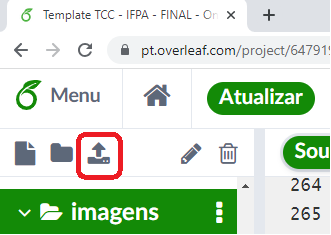
\includegraphics[scale=0.3]{Backup/up1.png}}; 
\node[] at (1, -3.5)  (a2) {
\includegraphics[scale=0.09]{Backup/up3a.png}};
\node[] at (5.5, -4)  (a3) {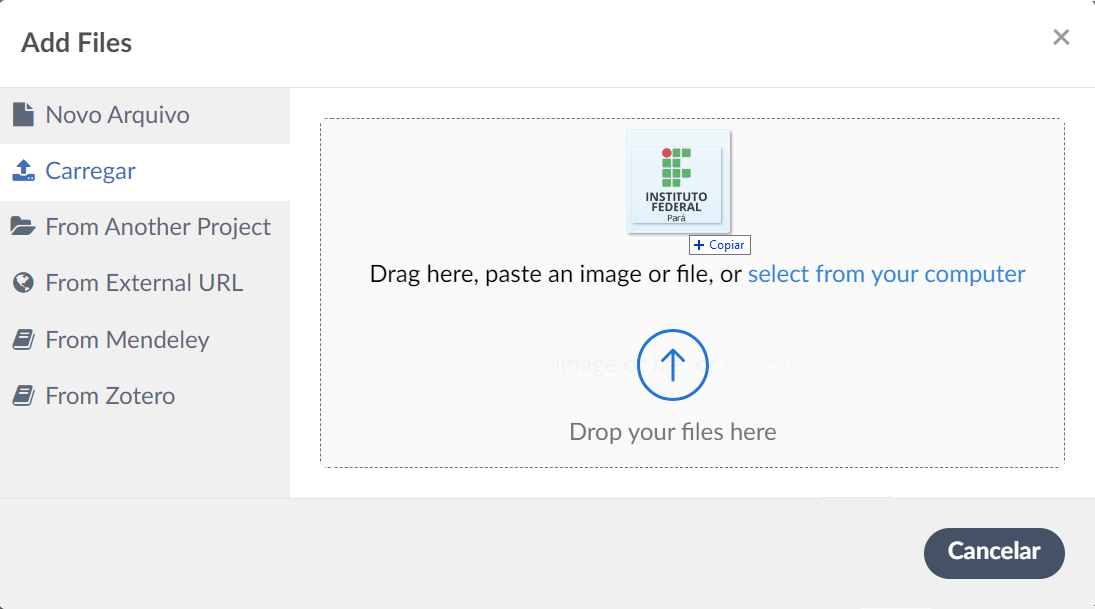
\includegraphics[scale=0.13]{Backup/up2.png}};
\node[] at (10.5, -4)  (a3) {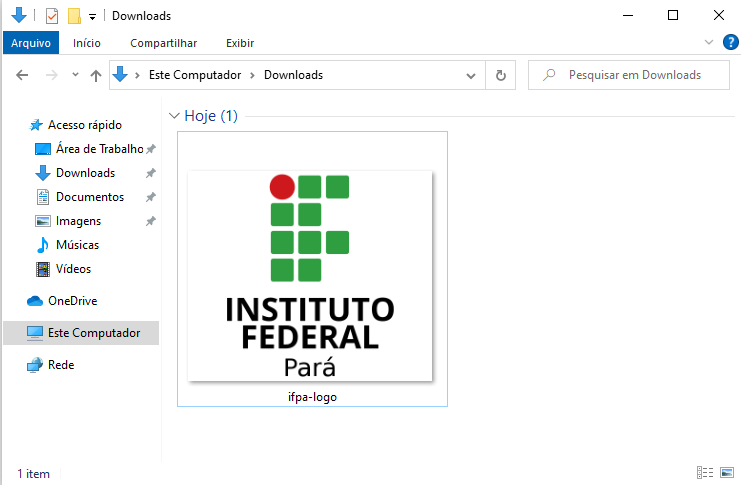
\includegraphics[scale=0.15]{Backup/up4.png}};
\node[] at (8.5, -3)  (a3) {
\includegraphics[scale=0.09]{Backup/up3b.png}};
\end{tikzpicture}
\end{tcolorbox}
}

\newcommand{\fazerLista}{
\begin{tcolorbox}[colback=blue!5!white,colframe=green!75!blue,title= Como criar uma lista numerada ou não]
Para criar uma Lista não numerada siga os passos abaixo:\\[5pt] 
\textcolor{blue}{$\backslash$begin}\{itemize\} \texttt{ - Inicia o ambiente lista}\\
\textcolor{blue}{$\backslash$item} primeiro\\ 
\textcolor{blue}{$\backslash$item} segundo\\
\textcolor{blue}{$\backslash$end}\{itemize\} \texttt{ - Finaliza o ambiente lista}\\[5pt]
\texttt{você deverá digitar o primeiro elemento da sua lista depois do comando  ``$\backslash$item''. Para acrescentar mais itens, após o ``Enter'' digite ``$\backslash$item'' antes do seu texto}
 \begin{multicols}{2}
Sua lista terá a aparência a seguir
\begin{itemize}
\item primeiro
\item segundo
\end{itemize}

\columnbreak
mudando o rótulo: \\\textcolor{blue}{$\backslash$begin}\{itemize\}[label=\textcolor{blue}{$\backslash$ding}\{42\}]
\begin{itemize}[label=\ding{42}]
\item primeiro
\item segundo
\end{itemize}
\end{multicols}
\textcolor{green!70!black}{Para mais rótulos, no Google procure \textit{pifont table}}\\[5pt]
Para criar uma Lista não numerada\\
\textcolor{blue}{$\backslash$begin}\{enumerate\} \texttt{ - Inicia o ambiente lista enumerada}\\
\textcolor{blue}{$\backslash$item} primeiro\\ 
\textcolor{blue}{$\backslash$item} segundo\\
\textcolor{blue}{$\backslash$end}\{enumerate\} \texttt{ - Finaliza o ambiente lista enumerada}
\begin{multicols}{2}
Sua lista terá a aparência a seguir
\begin{enumerate}
\item primeiro
\item segundo
\end{enumerate}

\columnbreak
mudando o rótulo: \\\textcolor{blue}{$\backslash$begin}\{enumerate\}[label=(\textcolor{blue}{$\backslash$alph*})]
\begin{enumerate}[label=(\alph*)]
\item primeiro
\item segundo
\end{enumerate}
\end{multicols}
\end{tcolorbox}
}

\newcommand{\adicionaCodigo}{
\begin{tcolorbox}[colback=blue!5!white,colframe=green!75!blue,title= Comando Adiciona Código, fontlower=\footnotesize]
Para adicionar código de uma linguagem de programação, siga os passos abaixo:\\[5pt] 
\textcolor{blue}{$\backslash$begin}\{lstlisting\}[language=\{\textcolor{blue}{NomeLinguagem}\}, caption=\{\textcolor{blue}{Nome Do Código}\}] \\ \texttt{ - Inicia o ambiente de código \\ Informa a Linguagem de Programação \\ Informa o título do código}\\
Código da Linguagem de Programação\\
\textcolor{blue}{$\backslash$end}\{lstlisting\}\texttt{ - finalização do ambiente de código}
\tcblower
\textcolor{blue}{EXEMPLO}\\
$\backslash$begin\{lstlisting\}[language=Python, caption=HelloWorld]\\
\tab print("Ola, Mundo")\\
$\backslash$end\{lstlisting\}\\
\end{tcolorbox}
}


%% \adicionaSigla
\newcommand{\adicionaSigla}{
\begin{tcolorbox}[colback=blue!5!white,colframe=green!75!blue,title= Comando Adiciona Sigla, fontlower=\footnotesize]
Para adicionar uma Sigla importante ao Texto e que deverá aparecer na \textcolor{blue}{Lista de Siglas e Abreviações}, siga os passos abaixo:\\[5pt] 
\textcolor{blue}{1 - Acesse o arquivo \{Escritor$\backslash$abreviaçõesSiglas.tex\}} \\[5pt]
\textcolor{blue}{EXEMPLO}\\[5pt]
\textcolor{blue}{$\backslash$DeclareAcronym}\{sbc\}\{\\
\texttt{Comando gerador de sigla \{ palavraChaveSigla \}}\\
\tab short = \normalfont{SBC}, \texttt{A Sigla como aparecerá}\\
\tab short-plural = s, \texttt{Sigla no modo plural (adição de s)}\\
\tab long  = Sociedade Brasileira de Computação, \texttt{por Extenso}\\
\tab tag = abbrev \texttt{abbrev - indicativo de SIGLA}\\
\} \texttt{- Fim da declaração de Sigla}\\[5pt]
\textcolor{blue}{2 - Faça referência à Sigla no Texto}
\tcblower
\textcolor{blue}{EXEMPLO}\\
\texttt{Teremos 2 comandos}\\[5pt]
\textcolor{blue}{$\backslash$ac}\{palavraChaveSigla\}\\
\texttt{Usado para mostrar a SIGLA literal}\\
\textcolor{blue}{$\backslash$acl}\{palavraChaveSigla\}\\
\texttt{Usado para mostrar a forma extensa da Sigla}\\
\textcolor{blue}{EXEMPLO}\\[5pt]
$\backslash$ac\{sbc\}\\
$\backslash$acl\{sbc\}\\
\\[5pt]
\textcolor{blue}{SBC}\\
\textcolor{blue}{Sociedade Brasileira de Computação}
\end{tcolorbox}
}


%% \adicionaSimbolo
\newcommand{\adicionaSimbolo}{
\begin{tcolorbox}[colback=blue!5!white,colframe=green!75!blue,title= Comando Adiciona Símbolo, fontlower=\footnotesize]
Para adicionar um Símbolo importante ao texto e que deverá aparecer na \textcolor{blue}{Lista de Símbolos}, siga os passos abaixo:\\[5pt] 
\textcolor{blue}{1 - Acesse o arquivo \{Escritor$\backslash$simbolos.tex\}} \\[5pt]
\textcolor{blue}{EXEMPLO}\\[5pt]
\textcolor{blue}{$\backslash$DeclareAcronym}\{megaByte\}\{\\
\texttt{Comando gerador de símbolo \{ palavraChaveSigla \}}\\
\tab short = \normalfont{MB}, \texttt{O Símbolo como aparecerá}\\
\tab long  = é uma unidade de medida de informação,\\
\tab \texttt{Significado do Símbolo por Extenso}\\
\tab sort  = MB, \texttt{Letra usada para ORDENAR na lista}\\
\tab tag = nomen \texttt{nomen- indicativo de SÍMBOLO}\\
\} \texttt{- Fim da declaração de Símbolo}\\[5pt]
\textcolor{blue}{2 - Faça referência ao Símbolo no Texto}
\tcblower
\textcolor{blue}{EXEMPLO}\\
\texttt{Teremos 2 comandos}\\[5pt]
\textcolor{blue}{$\backslash$ac}\{palavraChaveSigla\}\\
\texttt{Usado para mostrar a SIGLA literal}\\
\textcolor{blue}{$\backslash$acl}\{palavraChaveSigla\}\\
\texttt{Usado para mostrar a forma extensa da Sigla}\\
\textcolor{blue}{EXEMPLO}\\[5pt]
$\backslash$ac\{megaByte\}\\
$\backslash$acl\{megaByte\}\\
\\[5pt]
\textcolor{blue}{MB}\\
\textcolor{blue}{é uma unidade de medida de informação}
\end{tcolorbox}
}

%% \adicionaPalavraGlossario
\newcommand{\adicionaPalavraGlossario}{
\begin{tcolorbox}[colback=blue!5!white,colframe=green!75!blue,title= Comando Adiciona Palavras ao Glossário, fontlower=\footnotesize]
Para adicionar uma Palavra que é importante ao texto e que deverá aparecer no \textcolor{blue}{Glossário}, siga os passos abaixo:\\[5pt] 
\textcolor{blue}{1 - Acesse o arquivo \{Escritor$\backslash$glossario.tex\}} \\[5pt]
\textcolor{blue}{EXEMPLO}\\[5pt]
\textcolor{blue}{$\backslash$newglossaryentry}\{latex\}\{\\
\texttt{Gerador de Palavra do Glossário \{ palavraChaveGlossario \}}\\
\tab name = \{LATEX\}, \texttt{- Palavra como aparecerá no Glossário}\\
\tab text  = \{LaTeX\}, \texttt{- Como aparecerá no texto} \\
\tab sort = \{latex\}, \texttt{- Usado para Ordenar as palavra }\\
\tab description = \{É uma linguagem de marcação especialmente feita para documentos científicos\}, \\
\tab \texttt{Descrição por extenso da palavra - LaTeX}\\
\} \texttt{- Fim da declaração de Palavra do Glossário}\\[5pt]
\textcolor{blue}{2 - Faça referência à Palavra do Glossário no Texto} \\[5pt]
\textcolor{blue}{EXEMPLO}\\[5pt]
\texttt{Teremos 1 comando}\\[5pt]
\textcolor{blue}{$\backslash$gls}\{palavraChaveGlossário\}\\
\texttt{Usado para mostrar o texto da Palavra do Glossário}
\tcblower
\textcolor{blue}{EXEMPLO}\\
$\backslash$gls\{latex\}\\
\\[5pt]
\textcolor{blue}{LaTeX}\\
\end{tcolorbox}
}

%8888888888888888888888888888888888888888888888888888



% -------------------------------------------------
% Pacotes para QUDROS
% -------------------------------------------------
\newcommand{\quadroname}{Quadro}
\newcommand{\listofquadrosname}{Lista de Quadros}
\newfloat{Quadro}{\quadroname}{loq}[chapter]
\restylefloat*{Quadro}
\setfloatadjustment{Quadro}{\centering}
\setfloatlocations{Quadro}{hbtp}
\newlistof{listofquadros}{loq}{\listofquadrosname}
\newlistentry{Quadro}{loq}{0}
\counterwithout{Quadro}{chapter}
\renewcommand{\cftQuadroname}{\quadroname\space}
\renewcommand*{\cftQuadroaftersnum}{\hfill\textendash\hfill}


% -------------------------------------------------
% Configurações para aumentar a quantidade caracteres
% -------------------------------------------------
\tolerance=1
\emergencystretch=\maxdimen
\hyphenpenalty=10000
\hbadness=10000

% -------------------------------------------------
% Configurações para definir um comando de espaço inical no parágrafo
% -------------------------------------------------
\newcommand\tab[1][1cm]{\hspace*{#1}}   
%%%%%       \tab

% -------------------------------------------------
% Configurações para Definir quais capítulos aparecerão
% -------------------------------------------------
\providecommand{\Dedicatoria}{}
\newcommand{\temDedicatoria}[1]{
\renewcommand{\Dedicatoria}{#1}
}

\providecommand{\Agradecimento}{}
\newcommand{\temAgradecimento}[1]{
\renewcommand{\Agradecimento}{#1}
}

\providecommand{\Epigrafe}{}
\newcommand{\temEpigrafe}[1]{
\renewcommand{\Epigrafe}{#1}
}

\providecommand{\Ilustracoes}{}
\newcommand{\temListadeIlustracoes}[1]{
\renewcommand{\Ilustracoes}{#1}
}

\providecommand{\Tabelas}{}
\newcommand{\temListadeTabelas}[1]{
\renewcommand{\Tabelas}{#1}
}

\providecommand{\LCodigos}{}
\newcommand{\temListadeCodigos}[1]{
\renewcommand{\LCodigos}{#1}
}

\providecommand{\LQuadros}{}
\newcommand{\temListadeQuadros}[1]{
\renewcommand{\LQuadros}{#1}
}

\providecommand{\Siglas}{}
\newcommand{\temListadeSiglas}[1]{
\renewcommand{\Siglas}{#1}
}

\providecommand{\Simbolos}{}
\newcommand{\temListadeSimbolos}[1]{
\renewcommand{\Simbolos}{#1}
}

\providecommand{\Glossario}{}
\newcommand{\temGlossario}[1]{
\renewcommand{\Glossario}{#1}
}

\providecommand{\Apendices}{}
\newcommand{\temApendices}[1]{
\renewcommand{\Apendices}{#1}
}

\providecommand{\Anexos}{}
\newcommand{\temAnexos}[1]{
\renewcommand{\Anexos}{#1}
}

\providecommand{\Indice}{}
\newcommand{\temIndice}[1]{
\renewcommand{\Indice}{#1}
}

\providecommand{\ExemploTexto}{}
\newcommand{\temExemploTexto}[1]{
\renewcommand{\ExemploTexto}{#1}
}

\newenvironment{citacaodireta}
{\begin{quotation}\fontsize{10}{10}\selectfont}%\footnotesize}%
{\end{quotation}}


%marca{X} para Sim, caso contrário {}
%PRÉ TEXTUAIS
\temDedicatoria{x}
\temAgradecimento{x}
\temEpigrafe{x}
\temListadeCodigos{x}
\temListadeQuadros{x}
\temListadeTabelas{x}
\temListadeIlustracoes{x}
\temListadeSiglas{x}
\temListadeSimbolos{x}

%PÓS TEXTUAIS
\temGlossario{x}
\temApendices{x}
\temAnexos{x}
\temIndice{x}

%BACKUP
\temExemploTexto{x}

\makeindex

\renewcommand{\baselinestretch}{1.5}
%%%%%   comente os capítulos indesejados para que não apareceçam

% ---------------------------------------------------
% INICIO DE DOCUMENTO
% ---------------------------------------------------
\begin{document}
    \Urlmuskip=0mu plus 1mu\relax

\noindent
\acuseall

% ---------------------------------------------------
% Seleciona o idioma do documento (conforme pacotes do babel)
%\selectlanguage{english}
\selectlanguage{brazil}

% ---------------------------------------------------
% Retira espaço extra obsoleto entre as frases.
\setstretch{1.5}    % espaçamento entre linhas
\frenchspacing      % espaçamento entre palavras

% ---------------------------------------------------
% configurações LSTLISTING
%\counterwithout{lstlisting}{chapter}


% ---------------------------------------------------
% ELEMENTOS PRÉ-TEXTUAIS
% ---------------------------------------------------
\pretextual


% ---
% Capa
\imprimircapa


% ---
% Folha de rosto
% (o * indica que haverá a ficha bibliográfica)
\imprimirfolhaderosto
% ---
% Inserir folha de aprovação
% Isto é um exemplo de Folha de aprovação, elemento obrigatório da NBR
% 14724/2011 (seção 4.2.1.3). Você pode utilizar este modelo até a aprovação
% do trabalho. Após isso, substitua todo o conteúdo deste arquivo por uma

\begin{folhadeaprovacao}
    \setcounter{page}{1}
    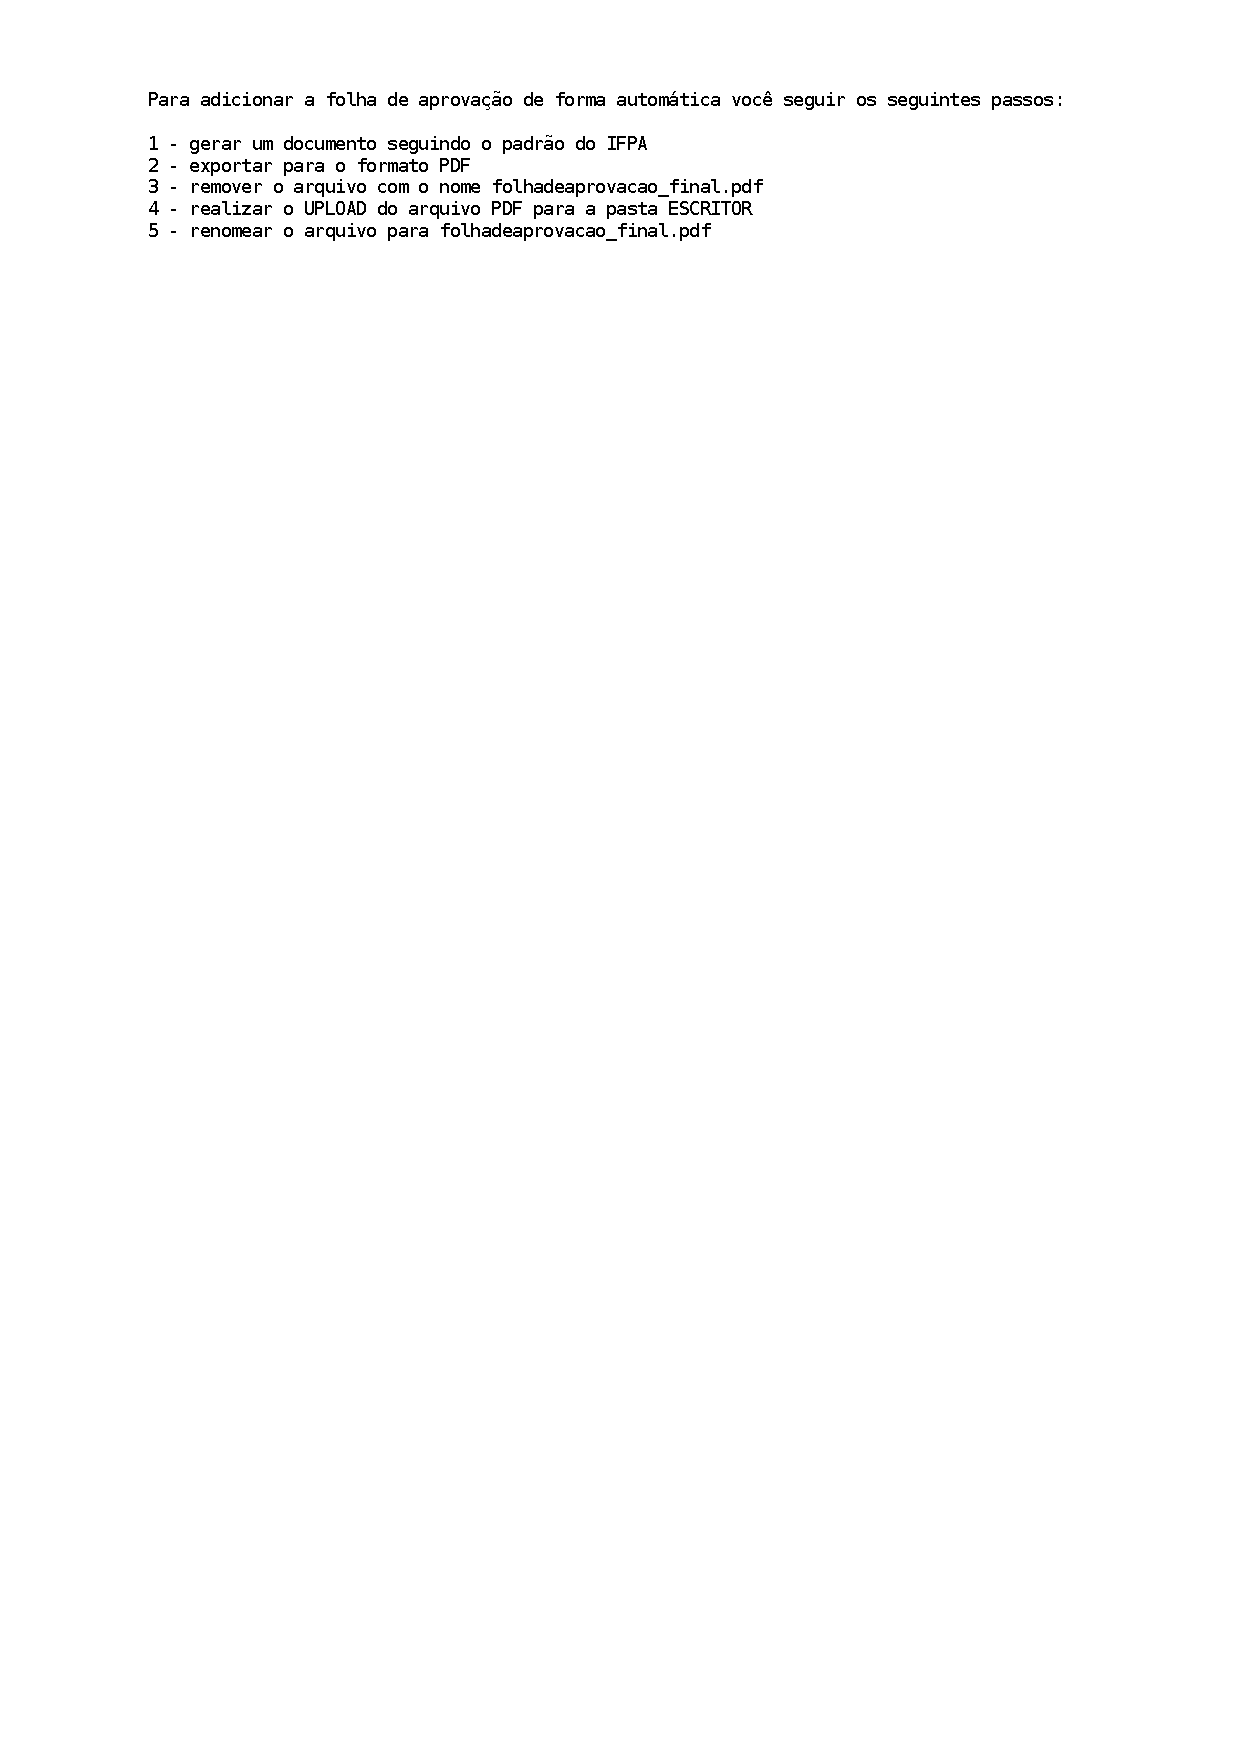
\includepdf[scale=0.95]{Escritor/folhadeaprovacao_final.pdf}
\end{folhadeaprovacao}

% ---
% Inserir folha de ficha catalográfica preparada pela biblioteca
\begin{folhadefichacatalografica}
    \setcounter{page}{1}
    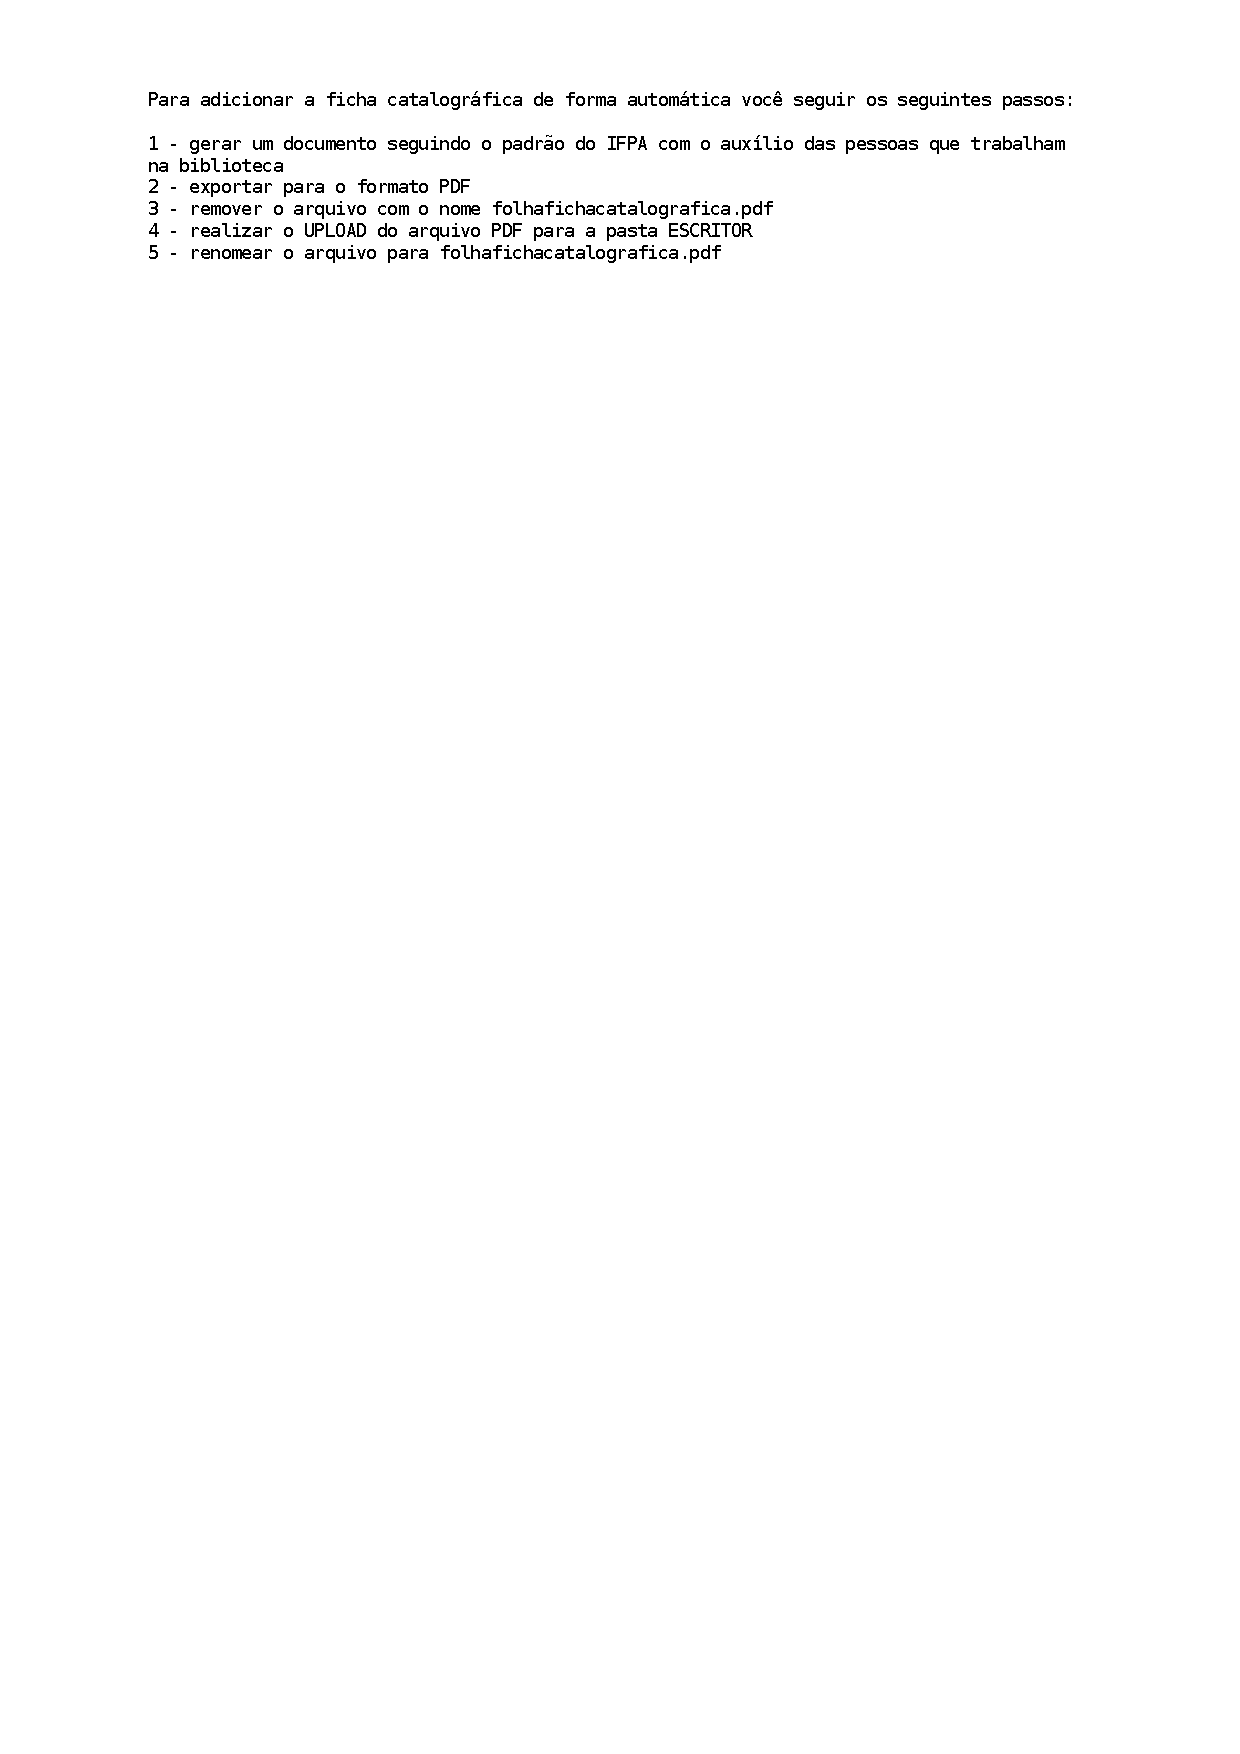
\includepdf[scale=0.95]{Escritor/folhafichacatalografica.pdf}
\end{folhadefichacatalografica}

% ---
% Dedicatória
\ifthenelse{\equal{\Dedicatoria}{}}{}{
\begin{dedicatoria}
    \normalsize
    \onehalfspacing
    \vspace*{\fill}
    \noindent
    \leftskip=7,5cm
    %%%%%%    Dedicatória
    
    Homenagem que o autor presta a uma ou mais pessoas.
%    \vspace{1cm}
\end{dedicatoria}
}

%%% AJUSTE DE MARGEM PARA ÁREA DO TEXTO
\setlength{\marginparwidth}{2cm}
\setlength{\marginparsep}{0cm}
\setlength{\headheight}{0cm}
\setlength{\headsep}{0.01cm}
\setlength{\topmargin}{-0.25cm}
% ---
% Agradecimentos
\ifthenelse{\equal{\Agradecimento}{}}{}{
\begin{agradecimentos}
    Agradecimentos dirigidos àqueles que contribuíram de maneira relevante à elaboração do trabalho, sejam eles pessoas ou mesmo organizações.
\newline
\newline
% para iniciar um novo agradecimento, ponha 2 comandos newline
Agradecimentos dirigidos àqueles que contribuíram de maneira relevante à elaboração do trabalho, sejam eles pessoas ou mesmo organizações.
\newline
\newline
% para iniciar um novo agradecimento, ponha 2 comandos newline
Agradecimentos dirigidos àqueles que contribuíram de maneira relevante à elaboração do trabalho, sejam eles pessoas ou mesmo organizações.
\end{agradecimentos}
}
% AJUSTE DE TEXTO DEPOIS
\setlength{\marginparwidth}{2cm}
\setlength{\marginparsep}{0cm}
\setlength{\headheight}{0.5cm}
\setlength{\headsep}{0.01cm}
\setlength{\topmargin}{0cm}

% ---
% Epígrafe
\ifthenelse{\equal{\Epigrafe}{}}{}{
\begin{epigrafe}
    \vspace*{\fill}
	\begin{flushright}
        %%%%  Toda a configuração está correta
%%%%  Se atenha a pôr uma epígrafe relacionada ao tema
%%%%
  
  \textit{Citação}

		Autor
	\end{flushright}
\end{epigrafe}
}

% ---
% RESUMOS
% resumo em português
\setlength{\absparsep}{18pt} % ajusta o espaçamento dos parágrafos do resumo
\begin{resumo}
    %NBR 6028 http://plone.ufpb.br/secretariado/contents/documentos/2021_ABNT6028Resumo.pdf
%4.1.8 Quanto à sua extensão, convém que os resumos tenham:
%a) 150 a 500 palavras nos trabalhos acadêmicos e relatórios técnicos e/ou científicos;
%b) 100 a 250 palavras nos artigos de periódicos;
%c) 50 a 100 palavras nos documentos não contemplados nas alíneas anteriores.

O resumo deve apresentar de forma concisa os pontos relevantes de um texto, fornecendo uma visão rápida e clara do conteúdo e das conclusões do trabalho. O texto, redigido na forma impessoal do verbo, é constituído de uma sequência de frases concisas e objetivas e não de uma simples enumeração de tópicos, não ultrapassando 500 palavras, seguido, logo abaixo, das palavras representativas do conteúdo do trabalho, isto é, palavras-chave e/ou descritores. Por exemplo, deve-se evitar, na redação do resumo, o uso de fórmulas, equações, diagramas e símbolos, optando-se, quando necessário, pela transcrição na forma extensa, além de não incluir citações bibliográficas.  Citação no rodapé normalmente utilizada para referenciar páginas Web.

\palavraschave{Palavra-chave 1; Palavra-chave 2; Palavra-chave 3}

Palavras-chave: \imprimirpalavraschave .    
\end{resumo}
\cleardoublepage

% ---
% ABSTRACT
% resumo em inglês
\renewcommand{\resumoname}{Abstract} 
\begin{resumo}
   This is the english abstract.

%\imprimirpalavraschave

\keywords{Keyword 1; Keyword 2; Keyword 3}

Keywords: \imprimirkeywords .
\end{resumo}
\cleardoublepage



%%% AJUSTE DE MARGEM PARA ÁREA DO TEXTO
\setlength{\marginparwidth}{2cm}
\setlength{\marginparsep}{0cm}
\setlength{\headheight}{0cm}
\setlength{\headsep}{0.01cm}
\setlength{\topmargin}{-0.25cm}


% ---
% inserir lista de códigos
\ifthenelse{\equal{\LCodigos}{}}{}{
\pdfbookmark[0]{\lstlistlistingname}{loc}
\lstlistoflistings
\cleardoublepage
}

% AJUSTE DE TEXTO DEPOIS
\setlength{\marginparwidth}{2cm}
\setlength{\marginparsep}{0cm}
\setlength{\headheight}{0.5cm}
\setlength{\headsep}{0.01cm}
\setlength{\topmargin}{0cm}


% ---
% inserir lista de quadros
\ifthenelse{\equal{\LQuadros}{}}{}{
\counterwithout{Quadro}{chapter}
\pdfbookmark[0]{\listofquadrosname}{loq}
\renewcommand{\listofquadrosname}{\textbf{LISTA DE QUADROS}\vspace{7mm}}
\listofquadros*
\cleardoublepage
}

% ---
% inserir lista de tabelas
\ifthenelse{\equal{\Tabelas}{}}{}{
\pdfbookmark[0]{\listtablename}{lot}
\renewcommand{\listtablename}{\textbf{LISTA DE TABELAS}\vspace{7mm}}
\listoftables*
\cleardoublepage
}

% ---
% inserir lista de figuras
\ifthenelse{\equal{\Ilustracoes}{}}{}{
\pdfbookmark[0]{\listfigurename}{lof}
\renewcommand{\listfigurename}{\textbf{LISTA DE ILUSTRAÇÕES}\vspace{7mm}}
\listoffigures*
\cleardoublepage
}

%%% AJUSTE DE MARGEM PARA ÁREA DO TEXTO
\setlength{\marginparwidth}{2cm}
\setlength{\marginparsep}{0cm}
\setlength{\headheight}{0cm}
\setlength{\headsep}{0.01cm}
\setlength{\topmargin}{-0.25cm}
% ---
% inserir lista de abreviaturas e siglas
\ifthenelse{\equal{\Siglas}{}}{}{
\pdfbookmark[0]{\listadesiglasname}{}
\printacronyms[include=abbrev, name=\listadesiglasname]
\cleardoublepage
}

% ---
% inserir lista de símbolos
\ifthenelse{\equal{\Simbolos}{}}{}{
\pdfbookmark[0]{\listadesimbolosname}{}
\printacronyms[name=\listadesimbolosname, exclude=abbrev]
\cleardoublepage
}
% AJUSTE DE TEXTO DEPOIS
\setlength{\marginparwidth}{2cm}
\setlength{\marginparsep}{0cm}
\setlength{\headheight}{0.5cm}
\setlength{\headsep}{0.01cm}
\setlength{\topmargin}{0cm}
% ---
% inserir o sumario
\pdfbookmark[0]{\contentsname}{toc}
\singlespacing
\renewcommand{\contentsname}{\textbf{SUMÁRIO}\vspace{7mm}}
\addtocontents{toc}{\protect\setcounter{tocdepth}{-1}}
\tableofcontents*
\addtocontents{toc}{\protect\setcounter{tocdepth}{3}}
\cleardoublepage

% ---
% Configuração de como aparecem os capítulos
\titleformat{\chapter}
    {\normalfont\sffamily\bfseries\MakeUppercase}{\thechapter}{0.5em}{}
\titlespacing{\chapter}{0em}{0em}{1.5em}

% AJUSTE DE TEXTO DEPOIS

\setlength{\headheight}{0.5cm}
\setlength{\headsep}{0.01cm}
\setlength{\topmargin}{0cm}

%% TOP
%\setlength{\headheight}{0.5cm}   % 5
%\setlength{\topmargin}{-0.5cm}   % 4
%\setlength{\headsep}{0.5cm}      % 6
\setlength{\headheight}{0.5cm}
\setlength{\headsep}{0.01cm}
\setlength{\topmargin}{0cm}

%% RIGHT
\setlength{\marginparwidth}{0cm}
\setlength{\marginparsep}{2cm}

%% TEXTO
\setlength{\textheight}{700pt}
\setlength{\textwidth}{452pt}

%%  TAMANHO DO PAPEL
\setlength{\paperwidth}{597pt}
\setlength{\paperheight}{845pt}

\setstretch{1.5}    % espaçamento entre linhas
\frenchspacing      % espaçamento entre palavras

\textual
    
    \ifthenelse{\equal{\ExemploTexto}{}}{
    \chapter{INTRODUÇÃO}
\label{sec:introdução}

%comente a próxixma linha quando não quizer a caixa de ajuda apareça
\ajuda

\adicionaFig

\adicionaQuadro

\adicionaTabela

\adicionaCodigo

\adicionaSigla

\adicionaSimbolo

\adicionaPalavraGlossario


% Escreva sua introdução
    % ---
% Capítulo 2
% ---
\chapter{FUNDAMENTOS}
\label{sec:fundamentos}


    % ---
% Capítulo 3
% ---
\chapter{CAPÍTULO 3}
\label{sec:cap3}


    
% - - -
% Capítulo 4
% - - -
\chapter{CITAÇÕES}
\label{sec:citacoes}


    % - - -
% Capítulo 5
% - - -
\chapter{CAPÍTULO 5}
\label{sec:cap5}



    \chapter{CONSIDERAÇÕES FINAIS}
\label{sec:consideracoesfinais}
}{
    \chapter{INTRODUÇÃO}
\label{sec:introdução}

Para inicializar o primeiro parágrafo de uma seção utilize o padrão a seguir. A introdução é a parte inicial do texto e que possibilita uma visão geral de todo o trabalho, devendo constar a delimitação do assunto tratado, objetivos da pesquisa, motivação para o desenvolvimento da mesma e outros elementos necessários para situar o tema do trabalho.

    Qual o problema que você está tentando resolver através do trabalho? Quais as restrições de projeto envolvidas?

    Nesta seção, você deve descrever a situação ou o contexto geral referente ao assunto em questão, devem constar informações atualizadas visando a proporcionar maior consistência ao trabalho.

\section{Objetivos}

    Os objetivos constituem a finalidade de um trabalho científico, ou seja, a meta que se pretende atingir com a elaboração da pesquisa.
    
    Podemos distinguir dois tipos de objetivos em um trabalho científico:
    
    \begin{itemize}
        \item Objetivos gerais – são aqueles mais amplos. São as metas de longo alcance, as contribuições que se desejam oferecer com a execução da pesquisa.

        \item Objetivos específicos – são a delimitação das metas mais específicas dentro do trabalho. São elas que, somadas, conduzirão ao desfecho do objetivo geral.
        
    \end{itemize}
    
    Como os objetivos indicam ação, recomenda-se que eles sejam definidos por meio de verbos, tais como analisar, avaliar, caracterizar, discutir, diagnosticar, investigar, implantar, pesquisar, realizar, determinar, etc.
    
\section{Organização do Trabalho}

    Nesta seção deve ser apresentado como está organizado o trabalho, sendo descrito, portanto, do que trata cada capítulo.

Nesta seção deve ser apresentado como está organizado o trabalho, sendo descrito, portanto, do que trata cada capítulo.

Nesta seção deve ser apresentado como está organizado o trabalho, sendo descrito, portanto, do que trata cada capítulo.

\subsection{Tamanho de Fonte para capítulo, seção e subseção}

    Elementos textuais

    - Fonte 12

    - Primária - caixa alta, com negrito
    
    - Secundária - caixa baixa, com negrito
    
    - Terciária - caixa baixa, sem negrito
    
    - Quaternária - caixa baixa, sem negrito
    
    - Espaçamento entre linhas simples.

Elementos pós-textuais

    - Fonte 12
    
    - Caixa alta
    
    - Com negrito.
    \chapter{FUNDAMENTOS}
\label{sec:fundamentos}


Este é o primeiro capítulo da parte central do trabalho, isto é, o desenvolvimento, a parte mais extensa de todo o trabalho. Geralmente o desenvolvimento é dividido em capítulos, cada um com seções e subseções, cujo tamanho e número de divisões variam em função da natureza do conteúdo do trabalho.

Em geral, a parte de desenvolvimento é subdividida em três capítulos:

\begin{itemize}
    \item \textit{referencial ou embasamento teórico} – texto no qual se deve apresentar os aspectos teóricos, isto é, os conceitos utilizados e a definição dos mesmos; nesta parte faz-se a revisão de literatura sobre o assunto, resumindo-se os resultados de estudos feitos por outros autores, cujas obras citadas e consultadas devem constar nas referências;

    \item \textit{metodologia do trabalho ou procedimentos metodológicos} – deve constar o instrumental, os métodos e as técnicas aplicados para a elaboração do trabalho;

    \item \textit{resultados} – devem ser apresentados, de forma objetiva, precisa e clara, tanto os resultados positivos quanto os negativos que foram obtidos com o desenvolvimento do trabalho, sendo feita uma discussão que consiste na avaliação circunstanciada, na qual se estabelecem relações, deduções e generalizações.

\end{itemize}

É recomendável que o número total de páginas referente à parte de desenvolvimento não ultrapasse 60 (sessenta) páginas.

\section{Como Adicionar IMAGENS}

    Para adicionar uma imagem você deverá seguir o seguinte padrão.

\begin{lstlisting}[language=TeX, caption{Código da Imagem da Logo}, label{cod:logoIFPA}]
\begin{figure}[H]
    \setstretch{1.5}\centering\footnotesize
    \caption{Logo do IFPA}
    \begin{center}
        
\includegraphics[width=0.3\textwidth]{ifpa-logo.png}
    \end{center}
    \label{fig:logoIFPA}
    \par Fonte: Google Imagens
\end{figure}
\end{lstlisting}

\hfill

\begin{figure}[H]
    \setstretch{1.5}\centering\footnotesize
    \caption{Logo do IFPA}
    \begin{center}
        
\includegraphics[width=0.3\textwidth]{ifpa-logo.png}
    \end{center}
    \label{fig:logoIFPA}
    \par Fonte: Google Imagens
\end{figure}


\begin{lstlisting}[language=TeX, caption=Codigo da Imagem do Brasao]
\begin{figure}[H]
    \setstretch{1.5}\centering\footnotesize
    \caption{Brasão do Brasil}
    \begin{center}
        
\includegraphics[width=0.5\textwidth]{DeusAcimaDeTodos.png}
    \end{center}
    \label{fig:brasaoBrasil}
    \par Fonte: Google Imagens
\end{figure}
\end{lstlisting}

\hfill

\begin{figure}[H]
    \setstretch{1.5}\centering\footnotesize
    \caption{Brasão do Brasil}
    \begin{center}
        
\includegraphics[width=0.5\textwidth]{DeusAcimaDeTodos.png}
    \end{center}
    \label{fig:brasaoBrasil}
    \par Fonte: Google Imagens
\end{figure}

\begin{lstlisting}[language=TeX, caption=Codigo da Imagem do Album]
\begin{figure}[H]
    \setstretch{1.5}\centering\footnotesize
    \caption{Álbum A Presença da Glória da banda Santa Geração}
    \begin{center}
        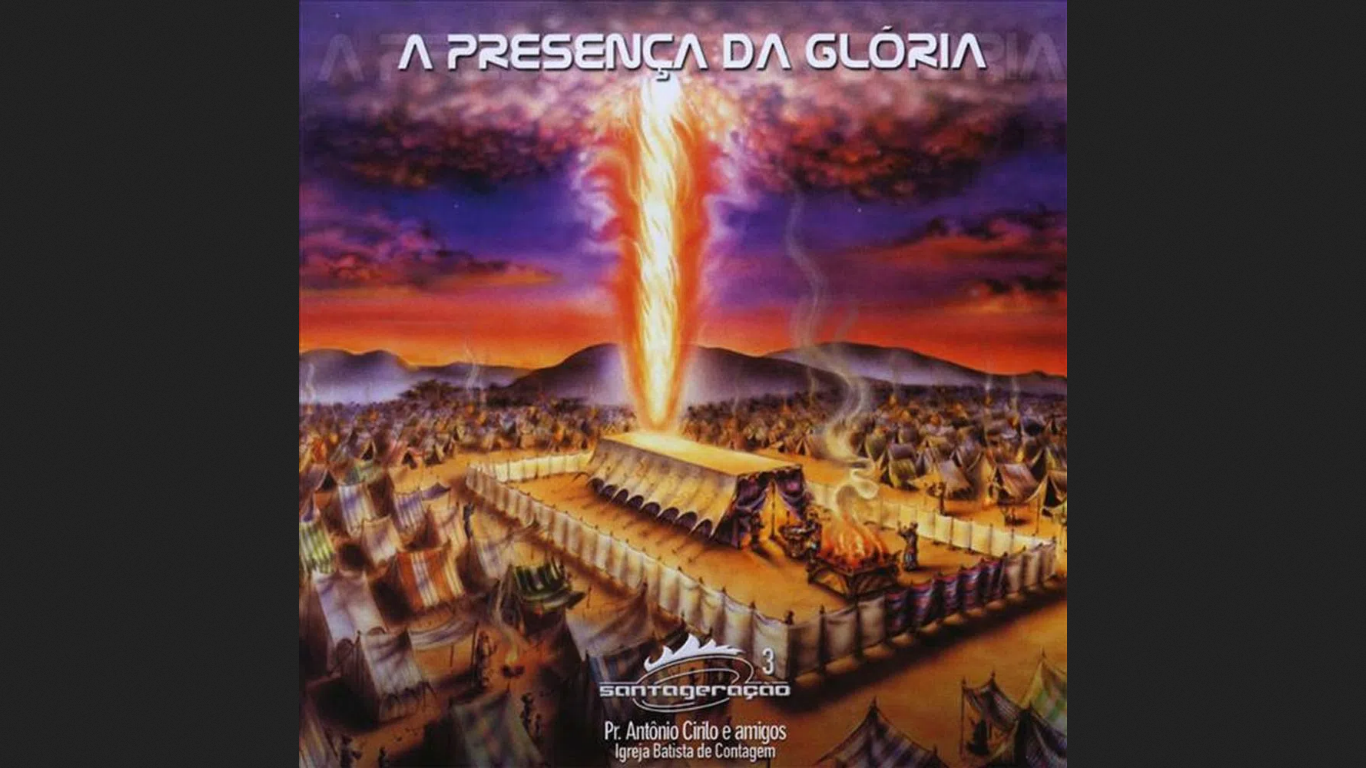
\includegraphics[width=0.5\textwidth]{presencaDaGloria.png}
    \end{center}
    \label{fig:capaPresencaDaGloria}
    \par Fonte: Google Imagens
\end{figure}
\end{lstlisting}

\begin{figure}[H]
    \setstretch{1.5}\centering\footnotesize
    \caption{Álbum A Presença da Glória da banda Santa Geração}
    \begin{center}
        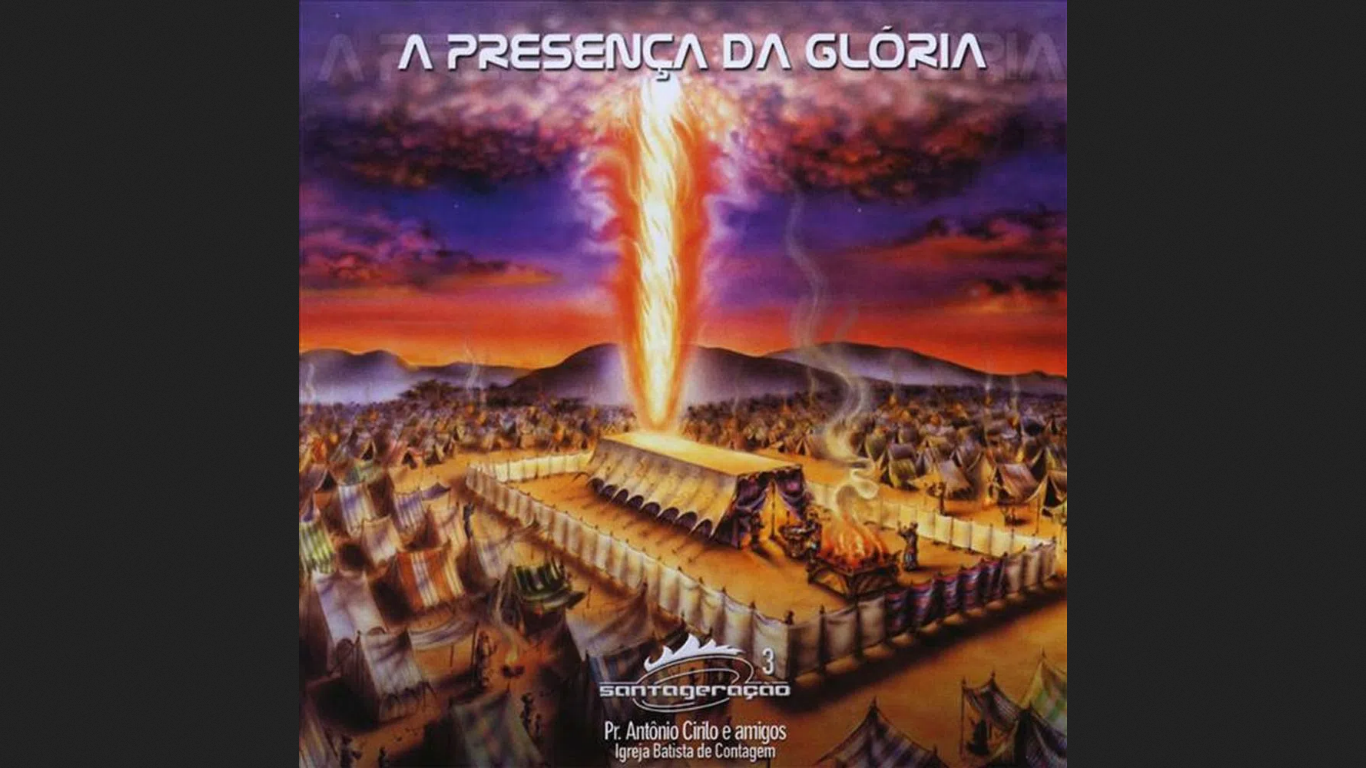
\includegraphics[width=0.5\textwidth]{presencaDaGloria.png}
    \end{center}
    \label{fig:capaPresencaDaGloria}
    \par Fonte: Google Imagens
\end{figure}
		
\section{Dando Nome e Referenciando Figuras no Texto}
	
Referenciamento da figura inserida na seção anterior: ~\autoref{fig:logoIFPA}.

\hfill

Comando:

\textbackslash ref\{fig:logoIFPA\}

\hfill

Esse referenciamento é possível devido ao padrão de inserção de imagem sugerido neste documento, o qual um dos campos da imagem é o \textbackslash capition acompanhado do \textbackslash label , onde definimos como poderemos referenciar tal imagem no decorrer do texto.

\hfill

\textbackslash label\{ fig:NomeDaFigura \}

\hfill

No campo \"NomeDaFigura\" podemos definir como iremos referenciar tal imagem no decorrer do texto usando o comando \textbackslash ref\{ fig:NomeDaFigura \}

\section{Abreviaturas e Simbolos}

Para utilizar abreviaturas e simbolos, basta utilizar o comando barra $\backslash$ combinado com ac ou acl.

Dentro das chaves você deve adicionar a palavra-chave da abreviatura ou símbolo

$\backslash$ac \{ \}

$\backslash$acl \{ \}

\hfill

Exemplo:

$\backslash$ac \{ abntex \}

AC \ac{abntex}.

$\backslash$acl \{ abntex \}

ACL \acl{abntex}.

\hfill

Simbolos e a versão por extenso.

$\backslash$ac \{ megaByte \}

\ac{megaByte}

$\backslash$acl \{ megaByte \}

\acl{megaByte}

\hfill

$\backslash$ac \{ lambda \}

AC \ac{lambda}.

$\backslash$acl \{ lambda \}

ACL \acl{lambda}.


\section{Glossário}

Para fazer uso do glossário (um elemento pós-textual), você deve usar o arquivo "glossário.tex" presente na pasta "Escritor", e seguir o exemplo que lá consta para adicionar as SUAS palavras que deverão constar no glossário.

No decorrer do texto você deverá usar o padrão \gls{fórmula} para marcar as palavras no momento conveniente do texto em que estas deverão aparecer.

Com isso, somente as palavras que você marcou usando o comando \textbackslash gls\{\} irão aparecer.

\textbackslash gls\{ sample \}

\gls{sample}.

\hfill

\textbackslash gls\{ fórmula \}

\gls{fórmula}.
    \chapter{CAPÍTULO 3}
\label{sec:cap3}

Algumas regras devem ser observadas na redação da monografia:.

\begin{itemize}
    \item ser claro, preciso, direto, objetivo e conciso, utilizando frases curtas e evitando ordens inversas desnecessárias;
    
    \item construir períodos com no máximo duas ou três linhas, bem como parágrafos com cinco linhas cheias, em média, e no máximo oito (ou seja, não construir parágrafos e períodos muito longos, pois isso cansa o(s) leitor(es) e pode fazer com que ele(s) percam a linha de raciocínio desenvolvida);
    
    \item a simplicidade deve ser condição essencial do texto; a simplicidade do texto não implica necessariamente repetição de formas e frases desgastadas, uso exagerado de voz passiva (como será iniciado, será realizado), pobreza vocabular etc. Com palavras conhecidas de todos, é possível escrever de maneira original e criativa e produzir frases elegantes, variadas, fluentes e bem alinhavadas;
    
    \item adotar como norma a ordem direta, por ser aquela que conduz mais facilmente o leitor à essência do texto, dispensando detalhes irrelevantes e indo diretamente ao que interessa, sem rodeios (verborragias);

    \item não começar períodos ou parágrafos seguidos com a mesma palavra, nem usar repetidamente a mesma estrutura de frase;

    \item desprezar as longas descrições e relatar o fato no menor número possível de palavras;
    
    \item recorrer aos termos técnicos somente quando absolutamente indispensáveis e nesse caso colocar o seu significado entre parênteses (ou seja, não se deve admitir que todos os que lerão o trabalho já dispõem de algum conhecimento desenvolvido no mesmo);
    
    \item dispensar palavras e formas empoladas ou rebuscadas, que tentem transmitir ao leitor mera ideia de erudição;

    \item não perder de vista o universo vocabular do leitor, adotando a seguinte regra prática: nunca escrever o que não se diria;

    \item usar termos coloquiais ou de gíria com extrema parcimônia (ou mesmo nem serem utilizados) e apenas em casos muito especiais, para não darem ao leitor a ideia de vulgaridade e descaracterizar o trabalho;

    \item ser rigoroso na escolha das palavras do texto, desconfiando dos sinônimos perfeitos ou de termos que sirvam para todas as ocasiões;

    \item em geral, há uma palavra para definir uma situação;

    \item encadear o assunto de maneira suave e harmoniosa, evitando a criação de um texto onde os parágrafos se sucedem uns aos outros como compartimentos estanques, sem nenhuma fluência entre si;

    \item ter um extremo cuidado durante a redação do texto, principalmente com relação às regras gramaticais e ortográficas da língua;

    \item geralmente todo o texto é escrito na forma impessoal do verbo, não se utilizando, portanto, de termos em primeira pessoa, seja do plural ou do singular.

\end{itemize}

Continuação.

\section{Tabelas}

Teste de uma tabela:

\begin{lstlisting}[language=TeX, caption={Code Sem Sentido}]
\begin{Quadro}[H]
    \setstretch{1.5}\centering\footnotesize
    \caption{Quadro sem sentido.}
    \begin{center}
        \begin{tabular}{|c|c|}
            \hline
            \textbf{Título Coluna 1} & \textbf{Título Coluna 2}\\
            1 & 2 \\
            \hline
            X & Y \\
            \hline
            X & W \\
            \hline
        \end{tabular}
    \end{center}
    \label{qua:tabela-ssentido}
    \par Fonte: Elaborado pelo próprio autor.
\end{Quadro}
\end{lstlisting}


\begin{Quadro}[H]
    \setstretch{1.5}\centering\footnotesize
    \caption{Quadro sem sentido.}
    \begin{center}
        \begin{tabular}{|c|c|}
            \hline
            \textbf{Título Coluna 1} & \textbf{Título Coluna 2}\\
            1 & 2 \\
            \hline
            X & Y \\
            \hline
            X & W \\
            \hline
        \end{tabular}
    \end{center}
    \label{qua:tabela-ssentido}
    \par Fonte: Elaborado pelo próprio autor.
\end{Quadro}

\begin{lstlisting}[language=TeX, caption={Comunicação Code}]
\begin{Quadro}[H]
    \setstretch{1.5}\centering\footnotesize
    \caption{Comparação entre os padrões de comunicação sem fio.}
    \begin{center}
        \begin{tabular}{|c|c|c|}
            \hline
            \textbf{LAN sem fio} & \textbf{Frequência} & \textbf{Taxa de Transmissão}  \\ \hline
            {802.11b} & 2,4 a 2,485 GHz& 11 Mbps\\ \hline
            {802.11g} & 2,4 GHz e 5 GHz& 54 Mbps \\ \hline
            {802.11n} & 2,4 GHz e 5 GHz & 200 Mbps a 600 Mbps \\ \hline
            {LoRa} & 868, 433, 915, 902 e 928 MHz & 50 Kbps \\ \hline
        \end{tabular}
    \end{center}
    \label{qua:transmissaoSemFio}
    \par Fonte: Elaborado pelo próprio autor.
\end{Quadro}
\end{lstlisting}

\hfill

\begin{Quadro}[H]
    \setstretch{1.5}\centering\footnotesize
    \caption{Comparação entre os padrões de comunicação sem fio.}
    \begin{center}
        \begin{tabular}{|c|c|c|}
            \hline
            \textbf{LAN sem fio} & \textbf{Frequência} & \textbf{Taxa de Transmissão}  \\ \hline
            {802.11b} & 2,4 a 2,485 GHz& 11 Mbps\\ \hline
            {802.11g} & 2,4 GHz e 5 GHz& 54 Mbps \\ \hline
            {802.11n} & 2,4 GHz e 5 GHz & 200 Mbps a 600 Mbps \\ \hline
            {LoRa} & 868, 433, 915, 902 e 928 MHz & 50 Kbps \\ \hline
        \end{tabular}
    \end{center}
    \label{qua:transmissaoSemFio}
    \par Fonte: Elaborado pelo próprio autor.
\end{Quadro}

\begin{lstlisting}[language=TeX, caption={Cronograma Code}]
\begin{table}[H]
    \setstretch{1.5}\centering\footnotesize
    \caption{Cronograma}
    \begin{center}
        \begin{tabular}{p{0.8cm}S[table-format=0.1]S[table-format=0.1]S%
        [table-format=0.1]S[table-format=0.1]S[table-format=0.1]}
            \toprule
            {N\textdegree} & {Ano} & {Mula} & {\textit{Network Coding}} & %
            {\textit{Routing}} & {Simulador}
            \\
            \midrule
            {[1]} & {2012} & {Proteus} & {XOR} & \textit{store-and-forward}%
            & {aplicação real}   \\
            {[2]} & {2016} & {Ônibus} & {XOR} & \textit{store-and-forward}%
            & \textit{The ONE} \\ 
            {[3]} & {2016} & {Barco} & {XOR} & {ER, EOR, FCR, SWR} &%
            \textit{The ONE}   \\
            \bottomrule
        \end{tabular}
    \end{center}
    \label{table:cronogramaT}
    \par Fonte: Elaborado pelo próprio autor.
\end{table}
\end{lstlisting}


\begin{table}[H]
    \setstretch{1.5}\centering\footnotesize
    \caption{Cronograma}
    \begin{center}
        \begin{tabular}{p{0.8cm}S[table-format=0.1]S[table-format=0.1]S%
        [table-format=0.1]S[table-format=0.1]S[table-format=0.1]}
            \toprule
            {N\textdegree} & {Ano} & {Mula} & {\textit{Network Coding}} & %
            {\textit{Routing}} & {Simulador}
            \\
            \midrule
            {[1]} & {2012} & {Proteus} & {XOR} & \textit{store-and-forward}%
            & {aplicação real}   \\
            {[2]} & {2016} & {Ônibus} & {XOR} & \textit{store-and-forward}%
            & \textit{The ONE} \\ 
            {[3]} & {2016} & {Barco} & {XOR} & {ER, EOR, FCR, SWR} &%
            \textit{The ONE}   \\
            \bottomrule
        \end{tabular}
    \end{center}
    \label{table:cronogramaT}
    \par Fonte: Elaborado pelo próprio autor.
\end{table}


\begin{lstlisting}[language=TeX, caption={Trabalhos NC}]
\begin{table}[H]
    \setstretch{1.5}\centering\footnotesize
    \caption{Relação dos trabalhos }	
    \begin{center}
        \begin{tabular}{p{0.8cm}S[table-format=0.1]S[table-format=0.1]S%
        [table-format=0.1]S[table-format=0.1]S[table-format=0.1]}
            \toprule
            {N\textdegree} & {Ano} & {Mula} & {\textit{Network Coding}} & %
            {\textit{Routing}} & {Simulador}
            \\
            \midrule
            {[1]} & {2012} & {Proteus} & {XOR} & \textit{store-and-forward}%
            & {aplicação real}   \\
            {[2]} & {2016} & {Ônibus} & {XOR} & \textit{store-and-forward}%
            & \textit{The ONE} \\ 
            {[3]} & {2016} & {Barco} & {XOR} & {ER, EOR, FCR, SWR} &%
            \textit{The ONE}   \\
            \bottomrule
        \end{tabular}
    \end{center}
    \label{table:trabalhoMulaNC}
    \par Fonte: Elaborado pelo próprio autor.
\end{table}
\end{lstlisting}

\hfill

\begin{table}[H]
    \setstretch{1.5}\centering\footnotesize
    \caption{Relação dos trabalhos }	
    \begin{center}
        \begin{tabular}{p{0.8cm}S[table-format=0.1]S[table-format=0.1]S%
        [table-format=0.1]S[table-format=0.1]S[table-format=0.1]}
            \toprule
            {N\textdegree} & {Ano} & {Mula} & {\textit{Network Coding}} & %
            {\textit{Routing}} & {Simulador}
            \\
            \midrule
            {[1]} & {2012} & {Proteus} & {XOR} & \textit{store-and-forward}%
            & {aplicação real}   \\
            {[2]} & {2016} & {Ônibus} & {XOR} & \textit{store-and-forward}%
            & \textit{The ONE} \\ 
            {[3]} & {2016} & {Barco} & {XOR} & {ER, EOR, FCR, SWR} &%
            \textit{The ONE}   \\
            \bottomrule
        \end{tabular}
    \end{center}
    \label{table:trabalhoMulaNC}
    \par Fonte: Elaborado pelo próprio autor.
\end{table}

\section{Seção 2}

Seção 2.

    \chapter{CITAÇÕES}
\label{sec:citacoes}

\section{Citações}
    \subsection{Citações com autoria dada pelo título (cite) }

    Padrão de referência para citação implícita e explícita.
    
    Artigo \cite{negrão14}
    
    Livro \cite[p.~55]{higginbottom1998performance}.
    
    Livro \cite{kurose2013computer}.
    
    Relatório Técnico \cite{Scott2007}.
    
    Site \cite{Raspberry}.

\begin{lstlisting}[language=TeX, caption={citação1}]
Artigo \cite{negrão14}

Livro \cite[p.~55]{higginbottom1998performance}.

Livro \cite{kurose2013computer}.

Relatório Técnico \cite{Scott2007}.

Site \cite{Raspberry}.    
\end{lstlisting}

   \subsection{Referências citadas por outra fonte (apud)}
    
    Livro \apud{higginbottom1998performance}{kurose2013computer}.
    
    Relatório Técnico \apudonline{Scott2007}{negrão14}.

\begin{lstlisting}[language=TeX, caption={citação2}]
Livro \apud{higginbottom1998performance}{kurose2013computer}.

Relatório Técnico \apudonline{Scott2007}{negrão14}.
\end{lstlisting}

   \subsection{Citações Múltiplas}
    
    Artigo \cite{negrão14, higginbottom1998performance, kurose2013computer}.
    
    Relatório Técnico \citeonline{Scott2007, kurose2013computer}.

\begin{lstlisting}[language=TeX, caption={citação4}]
Artigo \cite{negrão14, higginbottom1998performance, kurose2013computer}.

Relatório Técnico \citeonline{Scott2007, kurose2013computer}.
\end{lstlisting}

\section{Referenciar seção, imagem, tabela}

    Use o barra \ acompanhado do ref e logo depois adicione o tipo:referencia. Referência da imagem da logo da UFAM \ref{fig:logoIFPA} acompanhada da seção de introdução \ref{sec:introdução} na página \pageref{fig:logoIFPA}.

\begin{lstlisting}[language=TeX, caption={Refenciando Elementos}]
Referenciando imagem  \ref{fig:logoIFPA}

Referenciando seção \ref{sec:introdução}

Referenciando página \pageref{fig:logoIFPA}
\end{lstlisting}

\section{Adicionando Código}

Para adicionar código usando a biblioteca lstlisting, você deverá recorrer ao seguinte padrão.

\begin{lstlisting}[language=TeX, caption={Adicionando Código em LaTeX}]
\begin{lstlisting}[language=TeX, caption={Adicionando Código em LaTeX}]

Código em Latex com citação \cite{kurose2013computer}.

\end{ lstlisting}    %%% SEM O ESPAÇO EM BRANCO
\end{lstlisting}

\begin{lstlisting}[language=TeX, caption={Adicionando Código - Como aparecerá}]

Código em Latex com citação \cite{kurose2013computer}.

\end{lstlisting}

\begin{lstlisting}[language=C, caption={HelloWorld.c - neste template}]
\begin{lstlisting}[language=C, caption={HelloWorld.c - neste template}]
#include<stdio.h>

void main(){
    printf("Ola Mundo");
}
\end{ lstlisting}    // SEM O ESPAÇO EM BRANCO
\end{lstlisting}

\begin{lstlisting}[language=C, caption={HelloWorld.c - Como aparecerá}]
#include<stdio.h>

void main(){
    printf("Ola Mundo");
}
\end{lstlisting}
    \chapter{CAPÍTULO 5}
\label{sec:cap5}

 \section{Seção 1}
	
		Seção 1.
	
	\section{Seção 2}
	
		Alguns exemplos de citação:

			
	\section{Seção 3}
	
		Seção 3
    \chapter{CONSIDERAÇÕES FINAIS}
\label{sec:consideracoesfinais}

As considerações finais formam a parte final (fechamento) do texto, sendo dito de forma resumida (1) o que foi desenvolvido no presente trabalho e quais os resultados do mesmo, (2) o que se pôde concluir após o desenvolvimento bem como as principais contribuições do trabalho, e (3) perspectivas para o desenvolvimento de trabalhos futuros. O texto referente às considerações finais do autor deve salientar a extensão e os resultados da contribuição do trabalho e os argumentos utilizados estar baseados em dados comprovados e fundamentados nos resultados e na discussão do texto, contendo deduções lógicas correspondentes aos objetivos do trabalho, propostos inicialmente.

Deve ser apresentado a conclusão da pesquisa com base no objetivo geral e nos objetivos específicos para \"amarrar bem\" o tema aos resultados pretendidos.
    }

  
    % ----------------------------------------------------------
    % ELEMENTOS PÓS-TEXTUAIS
    % ----------------------------------------------------------
    \postextual
\Spacing{1.5}

%%%% glossario
%\glsaddall

\newcommand{\bibtextitlecommand}[2]{%
    \ifthenelse{\equal{#1}{inproceedings}}{\normalfont{\textbf{#2} $[\ldots]$}}{}}

\citeoption{abnt-emphasize=bf}

\bibitemsep = \baselineskip

\titleformat{\chapter}
    {\centering\normalfont\sffamily\bfseries\MakeUppercase}{\thechapter}{0.5em}{}

\titlespacing{\chapter}{0em}{0em}{3em}
%%% AJUSTE DE MARGEM PARA ÁREA DO TEXTO
\setlength{\marginparwidth}{2cm}
\setlength{\marginparsep}{0cm}


%\setlength{\headheight}{0.25cm}  % 5
%\setlength{\headsep}{0.1cm}    % 6
%\setlength{\topmargin}{-0.25cm} % 4

%\setlength{\headheight}{0.5cm}
%\setlength{\headsep}{0.01cm}
%\setlength{\topmargin}{0cm}

%\setlength{\headheight}{0cm}
%\setlength{\headsep}{0.01cm}
%\setlength{\topmargin}{-0.25cm}

    % ----------------Referencias Bibliograficas------------------------
    \bibliography{referencias}
    
    \setlength{\headheight}{0cm}
\setlength{\headsep}{0.01cm}
\setlength{\topmargin}{-0.25cm}

% -----------------------Glossário-----------------------------------
\ifthenelse{\equal{\Glossario}{}}{}{
\glsaddall
\chapter*{GLOSSÁRIO}
\addcontentsline{toc}{chapter}{\hspace{21mm}GLOSSÁRIO}
\setglossarysection{section}
\renewcommand{\glossarysection}[2][]{}
\printglossary
}

% -----------------------Apêndices--------------------------------
\ifthenelse{\equal{\Apendices}{}}{}{
\ifthenelse{\equal{\ExemploTexto}{}}
{% ---
% Inicia os apêndices
% ---
\begin{apendicesenv}

% ----------------------------------------------------------

%% adicione o seu conteúdo em apendice.tex
\addcontentsline{toc}{chapter}{\hspace{21mm}%
APÊNDICE A - Primeiro Apêndice}
\chapter*{Primeiro Apêndice}
\label{sec:apendicea}

Texto.

\addcontentsline{toc}{chapter}{\hspace{21mm}%
APÊNDICE B - Segundo Apêndice}
\chapter*{Segundo Apêndice}
\label{sec:apendiceb}

Texto.

% Comente a próxima linha
%\begin{apendicesenv}

% ----------------------------------------------------------

%% adicione o seu conteúdo em apendice.tex
\addcontentsline{toc}{chapter}{\hspace{21mm}%
APÊNDICE A - Primeiro Apêndice}
\chapter*{Primeiro Apêndice}
\label{sec:apendicea}

Os apêndices são textos ou documentos elaborados pelo autor, a fim de complementar sua argumentação, sem prejuízo da unidade nuclear do trabalho.

\addcontentsline{toc}{chapter}{\hspace{21mm}%
APÊNDICE B - Segundo Apêndice}
\chapter*{Segundo Apêndice}
\label{sec:apendiceb}

Texto.



\end{apendicesenv}



\end{apendicesenv}}{\begin{apendicesenv}

% ----------------------------------------------------------

%% adicione o seu conteúdo em apendice.tex
\addcontentsline{toc}{chapter}{\hspace{21mm}%
APÊNDICE A - Primeiro Apêndice}
\chapter*{Primeiro Apêndice}
\label{sec:apendicea}

Os apêndices são textos ou documentos elaborados pelo autor, a fim de complementar sua argumentação, sem prejuízo da unidade nuclear do trabalho.

\addcontentsline{toc}{chapter}{\hspace{21mm}%
APÊNDICE B - Segundo Apêndice}
\chapter*{Segundo Apêndice}
\label{sec:apendiceb}

Texto.



\end{apendicesenv}

}
}

% ------------------------Anexos-------------------------------
\ifthenelse{\equal{\Anexos}{}}{}{
% Anexos
% ----------------------------------------------------------

% ---
% Inicia os anexos
% ---
\begin{anexosenv}

% ---

% ---

% Adicione o seu conteúdo em anexo
\addcontentsline{toc}{chapter}{\hspace{21mm}ANEXO A - Primeiro Anexo}
\chapter*{ANEXO A - Primeiro Anexo}
\label{sec:anexoa}

Texto.


\addcontentsline{toc}{chapter}{\hspace{21mm}ANEXO B - Segundo Anexo}
\chapter*{ANEXO B - Segundo Anexo}
\label{sec:anexob}


Texto.



\end{anexosenv}
}
     
\end{document}